\documentclass[a4paper,12pt, german]{article}
\usepackage[a4paper, left=2.5cm, right=2cm, top=2.3cm, bottom=3cm]{geometry} % kleinere Ränder
\usepackage[onehalfspacing]{setspace}
\usepackage{comment} % Zum Auskommentieren ganzer Codeblöcke
\usepackage{fancyhdr}
\pagestyle{fancy}
\fancyhf{}
\fancyhead[R]{\itshape \leftmark}
\cfoot{\thepage}

%% commenting macros

% use this to hide larger blocks of material:
\usepackage{xcolor}
\usepackage{amsmath,amssymb}

% Define colors for authors
\definecolor{johannescolor}{rgb}{0.2,0.6,0.6}
\definecolor{danjecolor}{rgb}{0,0.7,0}

% Define colors for general macros
\definecolor{todocolor}{rgb}{0.9,0.1,0.1}
\definecolor{changedcolor}{rgb}{0.42,0.27,0.57}
\definecolor{addedcolor}{rgb}{0.867,0.176,0.361}
\definecolor{sourcecolor}{rgb}{0.25,0.4,0.7}

% General comment macro
\newcommand{\nbc}[3]{
    {\colorbox{#3}{\bfseries\sffamily\scriptsize\textcolor{white}{#1}}}
    {\textcolor{#3}{\sf\small$\blacktriangleright$\textit{#2}$\blacktriangleleft$}}
}
\newcommand{\cbs}[3]{
    {\colorbox{#2}{\bfseries\sffamily\scriptsize\textcolor{white}{#1}}}
}
  
% Define individual comments for authors
\newcommand{\johannes}[1]{\nbc{Johannes}{#1}{johannescolor}}
\newcommand{\danje}[1]{\nbc{Danje}{#1}{danjecolor}}

% Define general helper macros
\newcommand{\todo}[2]{\nbc{TODO:#1}{#2}{todocolor}}
\newcommand{\changed}[1]{\nbc{CHANGED}{#1}{changedcolor}}
\newcommand{\added}[1]{\nbc{ADDED}{#1}{addedcolor}}
\newcommand{\source}[1]{\cbs{SOURCE MISSING}{sourcecolor}}

\newcommand{\redacted}[1]{\emph{[anonymized for review]}}
%\renewcommand{\redacted}[1]{#1}

% Use this to temporarily hide reviewing comments, todos, etc.:
%  \renewcommand{\jane}[1]{}
%  \renewcommand{\john}[1]{}

% Use this to make "changed" items appear normal:
%\renewcommand{\changed}[1]{#1}
%\renewcommand{\added}[1]{#1}
%\renewcommand{\todo}[1]{}

%% end commenting macros

% Umlaute in der Datei erlauben, auf deutsch umstellen
\usepackage[utf8]{inputenc}
%\usepackage[ngerman]{babel}
\usepackage[nottoc,numbib]{tocbibind}
%\usepackage{mathptmx} % Hier steckt Times drin
%\usepackage{fontspec}
%\setmainfont{Times New Roman}
\usepackage{xcolor}


% Mathesymbole und Ähnliches
\usepackage{amsmath}
\usepackage{mathpartir}
\usepackage{mathtools}
\usepackage{amssymb}
\usepackage{amsthm}
\usepackage{mdframed}
%\usepackage{microtype}
\usepackage{stmaryrd}
\newcommand{\blitz}{\textcolor{red}{\lightning}}
\usepackage{float}
\renewcommand{\phi}{\varphi}


% Für Code
\usepackage{listings}
\lstset{frame=l,
  language=Java,
  basicstyle={\small\ttfamily},
  numberstyle=\tiny\color{blue},
  keywordstyle=\color{purple},
  commentstyle=\small\color{gray},
  stringstyle=\color{orange},
  breaklines=true,
  tabsize=2
}

% Pseudocode
\usepackage[vlined, linesnumbered, ruled]{algorithm2e}
\SetKwComment{Comment}{/* }{*/}
%\SetKwInput{KwData}{Input}
%\SetKwInput{KwResult}{Output}
\IncMargin{1.5em}

% Abbildungen
\usepackage{tikz}
\usetikzlibrary{arrows,calc,shapes,positioning}
\usepackage{wrapfig}
\usepackage[labelfont=bf]{caption}

% quotation
\definecolor{citeblue2}{RGB}{44,107,165}
\definecolor{citeblue}{rgb}{0,0.25,0.5}
\RequirePackage{csquotes}
\usepackage[backend=biber, style=numeric]{biblatex}
%\usepackage[citecolor=black, urlcolor=black, linkcolor=black]{hyperref}
\usepackage[citecolor=citeblue, urlcolor=citeblue, linkcolor=citeblue]{hyperref}
\hypersetup{colorlinks=true}
\usepackage[english, nameinlink, noabbrev]{cleveref}

% Custom Makros
\newcommand{\bangle}[1]{\langle #1 \rangle}
\newcommand{\semsof}[1]{\ensuremath{\llbracket #1 \rrbracket}}
\newcommand{\impl}{\Rightarrow}
\newcommand{\reason}[1]{\qquad \mid #1}
\newcommand{\edge}{\ensuremath{(e,e')}}
\newcommand{\edgein}{\ensuremath{(e,e') \in }}
\newcommand{\defof}{\text{Def. of }~}
\newcommand{\inv}{\ensuremath{{-1}}}
\newcommand{\prf}{\mathcal{P}}
\newcommand{\catprf}{\ensuremath{\mathcal{P}^{CAT}}}

% Reelle, Natürliche, Ganze, Rationale Zahlen
\newcommand{\R}{\ensuremath{\mathbb{R}}}
\newcommand{\N}{\ensuremath{\mathbb{N}}}
\newcommand{\Z}{\ensuremath{\mathbb{Z}}}
\newcommand{\Q}{\ensuremath{\mathbb{Q}}}
\newcommand{\E}{\ensuremath{\mathbb{E}}}
\newcommand{\B}{\ensuremath{\mathfrak{B}}}
\newcommand{\C}{\ensuremath{\mathfrak{C}}}


% Kürzel für Basisrelationen
\definecolor{rfgreen}{rgb}{0.2,0.55,0.2}
\newcommand{\0}{\textsf{\upshape 0}} % \upshape ensures that the relations remain their look in lemmata and inferrules
\newcommand{\po}{\textsf{\upshape po}}
\newcommand{\co}{\textsf{\textcolor{orange}{\upshape co}}}
\newcommand{\rf}{\textsf{\textcolor{rfgreen}{\upshape rf}}}
\newcommand{\ext}{\textsf{\upshape ext}}
\newcommand{\rmw}{\textsf{\upshape rmw}}
\newcommand{\hb}{\textsf{\textcolor{purple}{\upshape hb}}}
\newcommand{\loc}{\textsf{\upshape loc}}
\newcommand{\fr}{\textsf{\textcolor{violet}{\upshape fr}}}
\newcommand{\id}{\textsf{\upshape id}}
\newcommand{\true}{\textit{true}}
\newcommand{\false}{\textit{false}}
\newcommand{\rel}{\bangle{rel}}

%\newcommand{\rel}[1]{\textsf{#1}}
\newcommand{\relI}{\textsf{\upshape I}}
\newcommand{\relW}{\textsf{\upshape [W]}}
\newcommand{\relR}{\textsf{\upshape [R]}}
\newcommand{\relr}{\textsf{\upshape r}}
\newcommand{\Relr}{\relr}
\newcommand{\rels}{\textsf{\upshape s}}
\newcommand{\Rels}{\rels}
\newcommand{\relt}{\textsf{\upshape t}}


% Definitionsboxen
\usepackage[most]{tcolorbox}
%\definecolor{darkgray}{RGB}{70,90,70}
\definecolor{examblue}{rgb}{0,0.2,0.55}
\newenvironment{defi}[1]{%
\begin{tcolorbox}[blanker, before skip=5pt, after skip = 5pt, colback=darkgray!5!white, colframe=darkgray!75!black, title={{\sffamily} \textbf{#1}}]
}{
\end{tcolorbox}}

%Regelboxen
\tcbset{
  mybox/.style={
    colback=white,
    colframe=gray!70,
    colbacktitle=white,
    boxrule=2.5pt,
    coltitle=gray,
    arc=0pt,
    %before skip=0pt,
    %after skip=0pt,
    enhanced,
    left=6pt, right=6pt, top=6pt, bottom=6pt,
    attach boxed title to top left={yshift=-3mm, xshift=5mm},
    boxed title style={
    size=title,
    colback=white,
    colframe=white,
    boxrule=0.1pt
  }
  }
}
\newenvironment{rules}[1]{%
\begin{tcolorbox}[mybox, title={ \textbf{#1}}]
\begin{mathpar}
}{
\end{mathpar}
\end{tcolorbox}}

% Formelboxen
\newenvironment{formel}[1]{%
\begin{tcolorbox}[colback=white, colframe=violet!85!black, title={\sffamily \textbf{#1}}]
}{
\end{tcolorbox}}


%\theoremstyle{definition}
\newtheorem{theorem}{Theorem}%[section]

\newtheorem{proposition}[theorem]{Proposition}%[section]
\crefname{proposition}{Proposition}{Propositions}

\newtheorem{property}[theorem]{Eigenschaft}%[section]
\crefname{property}{Eigenschaft}{Eigenschaften}

\newtheorem{lemma}[theorem]{Lemma}%[section]
\crefname{lemma}{Lemma}{Lemmata}

%\newtheorem{definition}{Definition}
\mdfdefinestyle{theoremstyle}{%
linecolor=red,middlelinewidth=2pt,%
frametitlerule=true,%
frametitlebackgroundcolor=darkgray!60,
frametitlerulewidth=1pt,
innertopmargin=\topskip,
}
\mdfsetup{skipabove=\topskip , skipbelow=\topskip}
\mdfdefinestyle{defistyle}{linecolor=darkgray, linewidth=2pt, roundcorner=15pt, frametitlebackgroundcolor=gray!40, frametitlefont=\bfseries, theoremtitlefont=\bfseries, innertopmargin=5pt}
\mdtheorem[style=defistyle, nobreak=true]{definition}[theorem]{Definition}%[section]
\crefname{definition}{definition}{definitions}
\let\olddefinition\definition
\renewcommand{\definition}{\crefalias{theorem}{definition}\olddefinition}



% Beispiele
\newcounter{excount}
%\theoremstyle{definition}
\newtheorem{exi}[excount]{Beispiel}
\crefname{example}{Beispiel}{Beispiele}
\newenvironment{example}[2]{%
\begin{tcolorbox}[colback=white, colframe=examblue!85!black, title={\begin{exi}\label{#2} \textbf{#1}\end{exi}}]
}{
\end{tcolorbox}}




% Für Vektoren
\newcommand{\myvec}[1]{\ensuremath{\begin{pmatrix}#1\end{pmatrix}}}
\def\spvec#1{\left(\vcenter{\halign{\hfil$##$\hfil\cr \spvecA#1;;}}\right)}
\def\spvecA#1;{\if;#1;\else #1\cr \expandafter \spvecA \fi}

\usepackage{lipsum}

% PDFs includen
\usepackage{pdfpages}

\usetikzlibrary{positioning}
\tikzstyle{white} = [circle, minimum width=0.4cm, text centered, draw=black, fill=white]
\tikzstyle{blank} = [minimum width=0.6cm, text centered]
\tikzstyle{gray} = [circle, minimum width=0.6cm, text centered, text=white, draw=black, fill=darkgray]
\tikzstyle{blue} = [circle, minimum width=0.6cm, text centered, text=black, draw=black, fill=cyan]
\tikzstyle{purple} = [circle, minimum width=0.6cm, text centered, text=white, draw=black, fill=purple]
\tikzstyle{edge} = [thick,>=stealth]
\tikzstyle{arrow} = [thick,-stealth]


\addbibresource{includes/quellen.bib}


\begin{document}



\includepdf{includes/Titelseite/build/title.pdf}


{
\thispagestyle{empty}
\hypersetup{linkcolor=black}
\tableofcontents
\thispagestyle{empty}
}

\vfill

\section*{Abstract}
In dieser Bachelorarbeit werden zwei polynomielle Algorithmen für das \textit{Uncapacitated Facility Location} Problem (\textit{UFLP}) auf Bäumen zunächst erklärt und dann auf ihre Korrektheit und Laufzeitkomplexität überprüft. Zudem werden die Bedeutung und der Kontext der Algorithmen erläutert und somit die Einordnung der Algorithmen und damit verbundenen Beweise ermöglicht. \\
Die Algorithmen werden zusammen mit einigen anderen Versionen des \textit{UFLP} auf ihre Gemeinsamkeiten überprüft, um Hinweise zu erlangen, welche Eigenschaften dazu führen, dass diese Versionen polynomiell lösbar sind. Als diese stellt sich vor allem die Nutzung einer festen, von der Topologie des Graphen abhängigen Reihenfolge, die höchstens polynomiell von der Eingabe abhängig ist, für die Ermittlung lokaler Lösungen heraus.

\pagebreak
\setcounter{page}{1}

\section{Einleitung}\label{sec:intro}
Das \textit{Facility Location Problem} ist ein relevantes Problem im Bereich Operations Research, in Welchem Klienten aus einer Menge $I$, sogenannten \glqq Facilities\grqq{} aus Menge $J$ zugeordnet werden müssen. Dabei spielen die Transportkosten zwischen jeweiligen Klienten und Facilities eine Rolle, genauso wie die Kosten die Facilities zu eröffnen. \\
Dieses Problem kennt viele mögliche Anwendungen \cite[122]{Cor+90}. Möchte man zum Beispiel planen, wo ein Unternehmen seine Logistikzentren platzieren sollte, oder an welchen Orten idealerweise Krankenhäuser gebaut werden sollten, kann dies als Instanz des \textit{Facility Location Problem} interpretiert werden.\\

In dieser Bachelorarbeit wird die Komplexität des \textit{Uncapacitated Facility Location Problem} auf Bäumen analysiert. Dazu wird zunächst in \cref{sec:problemstellung} das Problem genau definiert und eine Formulierung als ganzzahliges Lineares Programm (IP) erstellt.
Außerdem gibt es einen kurzen Überblick über den Stand der Wissenschaft und Literatur zu diesem Thema und angrenzenden Themen der Standorttheorie (\cref{sec:literatur}), bevor im Kern dieser Arbeit (\cref{sec:kolen,sec:cornuejols}) zwei Algorithmen erklärt, auf ihre Korrektheit überprüft und ihre Laufzeitkomplexität analysiert werden. Diese Algorithmen zeigen, dass das Problem auf Bäumen polynomiell lösbar ist. Für ein besseres Verständnis der Beweise und der benutzten Algorithmen wird ein Beispiel verwendet. Dieses ist in \Cref{ex:example} zu sehen. \\

Danach werden die Beweise in \cref{sec:kontext} in den Kontext der Literatur eingeordnet und weitere polynomiell lösbare Fälle des \textit{UFLP} aufgeführt. Abschließend wird aus den gewonnenen Einblicken abgeleitet, welche Eigenschaften bestimmte Varianten des \textit{UFLP} einfacher machen als den generellen Fall (\cref{sec:characteristics}) und ein Fazit gezogen (\cref{sec:fazit}). \\
Im Anhang finden sich außerdem einige theoretische Grundlagen die benötigt werden um die Arbeit nachvollziehen zu können.

\subsection{Auswahl der Algorithmen}
Die Algorithmen, die in dieser Arbeit behandelt werden sind der Algorithmus von Kolen \cite{Kol82} und der Algorithmus von Cornuejols et al. \cite{Cor+90}. Der Algorithmus von Kolen ist der älteste und am häufigsten zitierte Algorithmus für \textit{UFLP} auf Bäumen und basiert darauf, die Matrix der Nebenbedingungen in eine bestimmte Form zu bringen. \\
Der Algorithmus von Cornuejols et al. ist der früheste gefundene Algorithmus, der stattdessen einen rekursiven Ansatz verfolgt. Auch wenn es andere solche Algorithmen gibt (\cite{ShaFar01}, \cite{BilCos94}), ist dieser der älteste von ihnen und am anschaulichsten zu erklären. Somit wurden diese beiden Algorithmen ausgewählt und repräsentieren die unterschiedlichen Ansätze, wie das \textit{UFLP} auf Bäumen effizient gelöst werden kann.

\pagebreak

\section{Literaturüberblick}\label{sec:literatur}
Dieser Abschnitt soll einen kurzen Überblick darüber geben, welche Aspekte des \textit{UFLP} wo in der Literatur zu finden sind und wie die Historie des Problems aussieht. \\
Ein relativ aktueller Überblick über die Facetten des gesamten \textit{Facility Location} Problems findet sich in \cite{EisMar11}, wobei sich das zweite \cite{Ver11} und dreizehnte Kapitel \cite{LowWen11} als relevant für diese Arbeit erweisen, da sie sich mit dem \textit{UFLP} bzw. der Lösung dessen auseinandersetzen. \\

Das \textit{Uncapacitated Facility Location Problem} wird in der Literatur zunächst in den 1960er Jahren von u.a. \cite{KueHam63} und \cite{Bal66} erwähnt.
Zum Lösen des \textit{UFLP} gibt es zahlreiche Ansätze. Sehr weit verbreitet ist der Ansatz von Erlenkotter (\cite{Erl78}), welcher mithilfe des dualen LPs eine optimale Lösung ermittelt. Ein früherer Ansatz ist beispielsweise der \textit{branch-and-bound} Algorithmus von Efroymson und Ray (\cite{EfrRay66}). \\
Ein Algorithmus, der die optimale Lösung approximiert ist zum Beispiel in \cite{ByrAar07} mit einem Approximationsfaktor von $1,5$ für das metrische \textit{UFLP}. \\

Ein weiteres Sammelwerk zum \textit{Facility Location Problem} ist das Buch \textit{Discrete Location Theory} von Mirchandani und Francis \cite{MirFra90}. In Diesem werden, wie in \cite{EisMar11}, viele Aspekte der Standorttheorie aufgegriffen wie zum Beispiel auch \textit{Covering} Probleme oder das \textit{p-Median} Problem, welches nah mit dem \textit{UFLP} verwandt ist. \\
Das dritte Kapitel ist der Beitrag \textit{The Uncapacitated Facility Location Problem} von Cornuejols et al. \cite{Cor+90}, welches in dieser Arbeit häufiger zitiert wird. In diesem Beitrag wird das \textit{UFLP} eingehend behandelt und Aspekte wie Heuristiken zum Lösen des Problems und die strenge LP-Relaxierung beleuchtet. \\
Außerdem wird auf polynomiell lösbare Fälle des ansonsten $\mathcal{NP}$-vollständigen Problems hingewiesen, von denen einer das \textit{UFLP} auf Bäumen ist. Für dieses Problem wird ein polynomieller Algorithmus beschrieben, der das Problem zunächst auf \textit{Tree Partition} reduziert und dafür dann den Algorithmus von Bárány et al. \cite{Bar+86} nutzt. 
In diesem Abschnitt wird ebenfalls die Arbeit von Antoon Kolen \cite{Kol83} zitiert, der sowohl einen eigenen polynomiellen Algorithmus vorstellt, als auch zeigt, dass eine optimale Lösung für das \textit{UFLP} auf Bäumen mithilfe einer Aufteilung in Covering-Probleme funktionieren kann. In seinem Algorithmus nutzt Kolen den von ihm mitentwickelten Algorithmus von Hoffman et al. \cite{Hof+85}, der für eine Reihe von Problemen bestimmt ist. Diese Probleme zeichnen sich dadurch aus, dass sie eine Nebenbedingungsmatrix haben, die in \textit{standart greedy form} ist. Die Idee, dass dies für bestimmte Subbäume eines Baumes anwendbar ist, stammt von Tamir \cite{Tam83}. Eine Übersicht darüber welche Probleme mithilfe dieses Algorithmus gelöst werden können und wie Diese zusammenhängen findet sich in \cite{Kol82}. \\

Weitere Fälle des \textit{UFLP}, die polynomiell lösbar sind, werden in \cite{Cor+90} und \cite{Kin11} erwähnt. Diese sind eine Version des \textit{UFLP}, die äquivalent zum \textit{Economic Lot Size} Problem ist von Krarup und Bilde \cite{KraBil77} und eine Version von Jones et al. \cite{Jon+95}. Außerdem gibt es einen polynomiellen Algorithmus für \textit{UFLP} auf Serien-parallelen Graphen \cite{HasTam86} und einen noch nicht publizierten Algorithmus für das \textit{Capacitated Facility Location} Problem auf Graphen mit beschränkter Baumweite \cite{Hos21}.



\section{Problemstellung und Notation} \label{sec:problemstellung}

Es existiert eine Menge von möglichen Standorten $J = \{1,...,m\}$ und eine Menge zu erreichender Klienten $I = \{1,...,n\}$. Diese Klienten könnten zum Beispiel Patienten eines Krankenhauses oder Standorte eines Logistikunternehmens sein. Dabei ist nicht ausgeschlossen, dass ein Standort auch ein Klient sein kann. Es gilt also nicht automatisch $I \cap J = \emptyset$. \\
Zu den Standorten  und Klienten  werden die Kosten als Standortkosten $c_j \in \R_+$ für $j \in J$ und Transportkosten $t_{ij} \in \R_+$ für $i \in I, j \in J$ definiert.
Nun ist das Finden von optimalen Standorten Thema dieser Arbeit. Optimal bedeutet in diesem Kontext, dass die Summe der Standortkosten und die Transportkosten vom Klienten zum Standort, von dem sie versorgt werden, minimiert werden. Formal definiert lautet das Problem wie folgt: 

\begin{definition}[\textit{Uncapacitated Facility Location Problem}]\label{def:uflp}
\[\underset{Q \subseteq J, g:I \rightarrow Q}{\min} \sum_{j \in Q} c_j + \sum_{j \in Q} \sum_{i \in I: g(i) = j} t_{ij} \text{ ,} \]

wobei $Q \subseteq J$ die Menge der eröffneten Facilities ist und $g:I\rightarrow Q$ jedem Klienten eine geöffnete Facility zuordnet.
\end{definition}

\begin{wrapfigure}{l}{0.6\textwidth}
\begin{definition}[Integer LP des \textit{UFLP}]\label{def:uflp2}
\begin{align}
\min & \sum_{i\in I} \sum_{j\in J} t_{ij}y_{ij} + \sum_{j\in J} c_jx_j \\
\text{unter } &\sum_{j \in J} y_{ij} = 1 && \forall i \in I \\
& y_{ij} \leq x_j && \forall i \in I, j \in J \\
& x_j, y_{ij} \in \{0,1\} && \forall i \in I, j \in J 
\end{align}
\end{definition}\end{wrapfigure}

Eine andere Möglichkeit das Problem zu formulieren ist über binäre Entscheidungsvariablen. Hier ist~$x_j~=~1$, falls $j$ eröffnet wird, sonst $0$ und~$y_{ij} =~1$, wenn ein genutzter Standort $j$ den Klienten~$i$ versorgt, sonst~$0$.
 Es gelten die Nebenbedingungen, dass jeder Klient von genau einem Standort versorgt wird (2), ein Standort eröffnet sein muss, um Klienten versorgen zu können (3) und~$x_j$ und $y_{ij}$ ganzzahlig sein müssen (4). 

Diese Form wird auch als \textit{Ganzzahliges Lineares Programm} beziehungsweise \textit{Integer Linear Program} (IP) bezeichnet.
Da, wie im Literaturüberblick erwähnt, eine Einschränkung auf Bäume das Problem einfacher macht, wird das Problem noch entsprechend angepasst.

Um das \textit{FLP} auf Bäume zu beschränken, muss es zunächst als Graphenproblem definiert werden: \\
Man erhält in diesem Fall zusätzlich den Graphen $G=(V,E)$ als Eingabe, wobei die Transportkosten aus den Kanten des Graphen ermittelt werden. Die Klienten und möglichen Facilities sind an den Knoten platziert, weshalb die Knotenmenge als $V=V_I \cup V_J$ definiert werden kann, mit \[V_J = \{v_j \mid j \in J\}\text{, } V_I = \{v_i \mid i \in I\}.\] 
Die Transportwege zwischen den Standorten und Klienten sind die Kanten \[E = \{ \{v_i,v_j\} \mid i,j \in I\cup J: \text{ Es existiert ein direkter Transportweg zwischen $i$ und $j$}\}.\] Die Standortkosten $c_j$ können als Knotengewichte für $v_j \in V_j$ und die Transportkosten $t_{ij}$ als Kantengewichte für $\{v_i,v_j\} \in E$ interpretiert werden. \\
Da nicht immer Klienten und versorgende Facility eine gemeinsame Kante haben, werden die Transportkosten für diesen Fall wie folgt definiert: 

\begin{definition}[Transportkosten]
Seien $v_i,v_j \in V$ zwei Knoten im Baum und $P(v_i,v_j)$ der Pfad, der sie verbindet. Die Transportkosten zwischen $v_i$ und $v_j$ sind definiert als die Summe der Kosten aller Kanten in $P(v_i,v_j)$:
\[t_{ij} = \sum_{\{v_k,v_{k'}\} \in P(v_i,v_j)} t_{kk'}\]
\end{definition}
Bei der Einschränkung gilt nun, dass der Graph $G$ ein Baum sein muss \cite{Cor+90}. \\

In dieser Arbeit soll erörtert werden, warum diese Baumstruktur das \textit{UFLP} weniger komplex macht. Insbesondere die Beweise aus \cite{Cor+90} und \cite{Kol83} für die Komplexität werden erklärt und analysiert. Im nächsten Abschnitt folgt zunächst der Algorithmus von Antoon Kolen.


\pagebreak
\section{Beweis von Antoon Kolen}\label{sec:kolen}
Der erste Beweis wurde von Antoon Kolen im Jahr 1983 veröffentlicht \cite{Kol83} und nutzt einen von Kolen zusammen mit Hoffman und und Sakarovitch entwickelten und erst 1985 publizierten Algorithmus. Dieser ermöglicht das Lösen des dualen LPs in polynomieller Laufzeit, solange die Matrix der Nebenbedingungen $A \in \Z^{n\times m}$ eine bestimmte Form hat \cite{Hof+85}.
Kolen stellt dabei zunächst diese bestimmte Form her, indem das Problem umformuliert wird. Insbesondere wird für die Reihenfolge der Spalten und Zeilen jeweils eine Ordnung hergestellt. Genaueres beschreiben die \cref{sec:ord,sec:neighbor}.


\subsection{Algorithmus}
In diesem Abschnitt wird der Algorithmus beschrieben, der dem Beweis zugrunde liegt.
Mithilfe des \Cref{ex:example} werden die Schritte anschaulich dargestellt.

\begin{figure}[h]
\begin{example}{Graph mit Klienten und Facility-Standorten}{ex:example}
Dieses Beispiel wird in der Arbeit zur anschaulichen Erklärung der Algorithmen benutzt. In grau sind die Klienten und in blau die möglichen Locations dargestellt. Zudem sind neben den Kanten in schwarz die Transportkosten und neben den Standortknoten in blau die Standortkosten eingezeichnet. \\ 

\centering
\begin{tikzpicture}[node distance=2cm]
\node[client] (R) {$R$};
\node[location, below left of=R, label=315:$\textcolor{cyan}{2}$] (B) {$B$};
\node[client, below right of=R] (C) {$C$};
\node[client, below left of=B] (D) {$D$};
\node[location, below left of=C, label=east:$\textcolor{cyan}{2}$] (E) {$E$};
\node[location, below right of=C, label=west:$\textcolor{cyan}{2}$] (F) {$F$};

\draw[edge] (R) --node[above left] {$3$} (B);
\draw[edge] (R) --node[above right] {$2$} (C);
\draw[edge] (B) --node[above left] {$1$} (D);
\draw[edge] (C) --node[above left] {$1$} (E);
\draw[edge] (C) --node[above right] {$2$} (F);
\end{tikzpicture}
\[I = \{R,C,D\} \quad J=\{B,E,F\}\]
\end{example}
\end{figure}

Der Algorithmus lässt sich in vier Schritte gliedern. Zunächst wird eine Ordnung auf dem Graphen induziert, dann werden sogenannte \glqq Neighborhood Subtrees\grqq{} ermittelt.
Um im letzten Schritt dann den Algorithmus von Hofmann et al. anwenden zu können, wird vorher das IP umgeformt.

\subsubsection{Induzieren einer Ordnung}\label{sec:ord}
Im ersten Schritt wird eine Ordnung auf dem Graphen induziert, welche später die Reihenfolge der Spalten in der Nebenbedingungsmatrix bestimmt. Dafür wird zunächst ein beliebiger Wurzelknoten $v_r \in V$ ausgewählt. 

Alle Knoten werden nun absteigend nach ihren Transportkosten zu $r$ geordnet, \\also~$t_{ir}~\geq~\dots~\geq~t_{rr}~=~0$. \\
So entsteht eine Ordnung an dessen Ende die Wurzel steht: $v_i \leq ... \leq v_r$. \\
Für eine anschauliche Darstellung wird dies in \Cref{ex:indord} auf den Graphen aus \Cref{ex:example} angewendet. 
\begin{example}{Induzierte Ordnung}{ex:indord}
Induzierte Ordnung für das Beispiel in \Cref{ex:example}
, wobei $R$ als Wurzel gewählt wurde:\\
\[ t_{FR} = 4 \geq t_{DR} = 4 \geq t_{ER} = 3 \geq t_{BR}=3 \geq t_{CR} = 2 \geq t_{RR} = 0\]

\[F \leq D \leq E \leq B \leq C \leq R\]
\end{example} 

\noindent 
 Nach dieser Ordnung werden die Spalten in $A$ geordnet, welche für die möglichen Facility Locations stehen. Um zu determinieren welche Werte durch die Nebenbedingungsmatrix repräsentiert werden und in welcher Reihenfolge die Zeilen stehen, wird im nächsten Abschnitt das Konzept der \glqq Neighborhood Subtrees\grqq{} vorgestellt. \\

\subsubsection{Berechnung der Neighborhood Subtrees}\label{sec:neighbor}

Für jeden Klienten $i \in I$ werden die Transportkosten zu allen möglichen Facility Standorten ermittelt und anschließend geordnet. \\
Um Verwechslungen zu vermeiden werden diese Werte hier als Distanzen bezeichnet. Für jeden Klienten $i$ gibt es dann insgesamt diese $t(i)+1$  Distanzen:
\[s_{i1} = 0 \leq s_{i2} = t_{ij} \leq ... \leq s_{it(i)} = t_{ij'} \leq s_{it(i)+1} = \infty\]

\noindent \begin{minipage}[c]{0.49\textwidth} 
 wobei $j$ der nächste Standort an $i$ ist und $j'$ der am weitesten entfernte Standort von~$i$.
Der Wert $t(i)$  ist also die Nummer des am weitesten entfernten Location-Knotens.
Die Werte~$s_{i1} = 0$ und $s_{it(i)+1}$ werden hinzugefügt, sollten sie nicht schon vorhanden sein. Das kann für $s_{i1}$ der Fall sein, sollte $i \in J$ gelten. Für eine Anwendung, siehe \Cref{ex:distances}.\\

\end{minipage}\begin{minipage}[c]{0.03\textwidth}
\hfill
\end{minipage}\begin{minipage}[c]{0.48\textwidth}
\centering
\vspace*{-0cm}
\begin{example}{geordnete Distanzen}{ex:distances}
Für den Graphen aus \Cref{ex:example} gilt für Knoten $R$:
\[s_{R1} = 0, s_{R2} = 3, s_{R3} = 4, s_{R4} = \infty\]
\end{example}
\end{minipage} \\

\noindent Diese Distanzen werden ebenfalls zur Berechnung von \glqq Neighborhood Subtrees\grqq{} genutzt.

\begin{definition}[Neighborhood Subtrees]
Neighborhood Subtrees sind Mengen von Locations $T_{i,k}$ die nicht weiter von $i \in I$ entfernt sind, als die entsprechende Distanz $s_{ik}$ \cite{Kol83}. \\
Sei $i \in I$ und $k \in \{0,1,...,t(i)\}$. Der Neighborhood Subtree für $i$ und $k$ ist:
\[T_{i,k} = \{j \in J \mid t_{ji} \leq s_{ik} \}\]
\end{definition}

\noindent Da die Distanzen dadurch definiert sind, dass mindestens eine mögliche Location genau so weit von~$v_i$ entfernt ist, muss mit jeder größeren Distanz mindestens ein Knoten mehr im Neighborhood Subtree sein, als bei einer geringeren Distanz.

\begin{example}{Neighborhood Subtrees}{ex:subtrees}
Neighborhood Subtrees für die Klientenknoten aus \Cref{ex:example}:
\small
\begin{align*}
&\text{Knoten } A: && \text{Knoten } C: && \text{Knoten }D: \\
&T_{A,1} = \emptyset && T_{C,1} = \emptyset && T_{D,1} = \emptyset  \\
&T_{A,2} =\{B,E\} && T_{C,2} =\{E\} && T_{D,2} = \{B\} \\
&T_{A,3} = \{B,E,F\} && T_{C,3} = \{E,F\} && T_{D,3} = \{B,E\} \\
&&& T_{C,4} = \{B,E,F\} && T_{D,4} = \{B,E,F\}
\end{align*}
\end{example} 

\noindent Die Neighborhood Subtrees repräsentieren in $A$ die Reihen. Sie werden für das Anlegen der Matrix \textit{lexikographisch} aufsteigend geordnet. Die \textit{lexikographische Ordnung} ist wie folgt definiert: 

\begin{definition}[Lexikographische Ordnung]
Seien $T_1, T_2$ zwei Mengen.
\[T_1 \subseteq T_2 \Rightarrow T_1 \leq_{lex} T_2\]
Im Falle $T_1 \nsubseteq T_2$ und $T_2 \nsubseteq T_1$ betrachtet man
$t_1$, das größte Element in $T_1\setminus T_2$ und $t_2$, das größte Element in $T_2 \setminus T_1$. Es gilt:
\[t_1 < t_2 \Rightarrow T_1 \leq_{lex} T_2\]
\end{definition}

\noindent Um zu entscheiden, ob $t_1 < t_2$ wird in diesem Verfahren die induzierte Ordnung aus \cref{sec:ord} verwendet.

\begin{example}{Lexikographische Ordnung}{ex:lexord}
Für das Beispiel wird die lexikographische Ordnung der Neighborhood Subtrees berechnet.
	\begin{align*}
	T_{A,1} =  T_{C,1} = T_{D,1} = \emptyset & \leq_{lex} T_{C,2} = \{E\} \\
	 &\leq_{lex} T_{C,3} = \{E,F\} \\ 
	 &\leq_{lex} T_{D,2} = \{B\} \\ 
	 &\leq_{lex} T_{A,2} = T_{D,3} = \{B,E\} \\ 
	 &\leq_{lex} T_{A,3} = T_{C,4} = T_{D,4} = \{B,E,F\}
	\end{align*}
\end{example}

\noindent Nun kann die Matrix $A$ angelegt werden. Die induzierte Ordnung aus \cref{sec:ord} gibt die Reihenfolge der Spalten vor und die lexikographische Ordnung aus diesem Abschnitt die Reihenfolge der Zeilen. Sie ist wie folgt definiert: 

\[a_{ij}^k = \begin{cases} 1 \, \text{wenn } t_{ij} \leq s_{ik} \\
				0 \, \text{ sonst} 
		\end{cases} \text{\cite{Kol83}.}\]

\newpage
\subsubsection{Umformung des IP}\label{sec:umformunglp}

Nun kann man das IP für das \textit{UFLP} auf Bäumen umformen zu einem IP, das auf der Matrix $A$ basiert. Dazu werden die Werte $z_i^k \in \{0,1\}$ benötigt:
\[z_i^k = \begin{cases} 1 & i \text{ wird \textbf{nicht} von einer geöffneten Facility }j \\&\text{versorgt, für die } t_{ij} \leq s_{ik} \text{ gilt.} \\
0 & \text{sonst}
\end{cases}\]

\noindent Für die Zielfunktion bleibt die Summe der Standortkosten~$\sum_{j\in J} c_jx_j$ erhalten.
 
 \noindent \begin{wrapfigure}{l}{0.6\textwidth}
\vspace*{-0.4cm}
\begin{definition}[Subtree IP]\label{def:subtreelp}
\begin{align*}
\min && \sum_{j=1}^m c_jx_j + \sum_{i=1}^{n} \sum_{k=1}^{t(i)} & (s_{ik+1} - s_{ik}) z_i^k \\
\text{unter } && \sum_{j=1}^m a_{ij}^k x_j + z_i^k  \geq 1 & \quad i \in I, k\in \{1,...,t(i)\} \\
&& x_j  \in \{0,1\} & \quad \forall j \in J\\
&& z_i^k  \in \{0,1\} & \quad \forall i \in I, k \in \{1,...,t(i)\} 
\end{align*}
\end{definition}\end{wrapfigure} 

 Die Transportkosten allerdings werden nun über die Summe \[\sum_{i \in I} \sum_{k=1}^{t(i)} (s_{ik+1} - s_{ik}) z_i^k\] bestimmt. 
Diese berechnet für jeden Klienten die Summe der Transportkosten zur nächsten offenen Facility. Dafür wird für jeden Subtree die zusätzliche Distanz im Vergleich zum vorherigen aufsummiert werden, bis ein Subtree eine geöffnete Facility enthält. 
Die Nebenbedingungen \[x_j \in \{0,1\}\quad \forall j \in J\] bleiben erhalten und \[z_i^k \in \{0,1\} \quad \forall i \in I, k=1,...,t(i)\] kommen dazu. Die anderen Nebenbedingungen werden ersetzt durch 
\[\sum_{j\in J} a_{ij}^k x_j + z_i^k \geq 1 \quad i \in I, k = 1,...,t(i)\]
wobei diese dafür sorgt, dass jeder Klient von der nächsten geöffneten Facility versorgt wird. Die Matrix $A = (a_{ij}^k)$ ist somit eine $n^* \times m$-Matrix, wobei $n^* = \sum_{i \in I} t(i)$ die Anzahl der Neighborhood Subtrees ist. \\

\pagebreak

\begin{theorem}[\cite{Kol83}]\label{thm:lpeq}
Das Subtree LP aus \cref{def:subtreelp} ist äquivalent zu dem IP des \textit{UFLP} in \cref{def:uflp2}.
\end{theorem} 

\begin{proof} Das \cref{thm:lpeq} besagt, dass das Subtree IP aus \cref{def:subtreelp} und die Definition des \textit{UFLP} aus \cref{def:uflp2} äquivalent sind. Diese Aussage wird in \cite{Kol83} dadurch bewiesen, dass der beste Wert $v(x)$ einer Lösung $x \in \{0,1\}^m$ vom Subtree IP äquivalent zu einer des \textit{UFLP} ist. Eine Lösung $x$ lässt sich interpretieren als charakteristische Funktion für die Menge $Q$ aus \cref{def:uflp}. \\

Der beste Wert $v(x)$ für einen $(0,1)$-Vektor wird erreicht dadurch, dass jeder Klient durch die nächste geöffnete Facility versorgt wird. Somit gilt für eine Lösung $x$ des \textit{UFLP}:
\begin{equation}\label{eq:besterwert}v(x) = \sum_{j \in J} c_jx_j + \sum_{i \in I} \underset{j \in J: x_j=1}{\min} \{t_{ij}\}
\end{equation}

\noindent Sei $s_{il}$ die kürzeste Distanz von $i$ zu einer geöffneten Facility, also $s_{il} = \underset{j \in J:x_j = 1}{\min}\{t_{ij}\}$. Dann gilt:
\[\sum_{j\in J} a_{ij}^k x_j \geq 1 \quad \forall k \geq l \quad \text{ und } \quad \sum_{j\in J} a_{ij}^k x_j = 0 \quad \forall k <l\]

\noindent Somit ist für alle $k \geq l: z_i^k = 1$ und für alle $k < l: z_i^k =1$ die minimale Lösung und erzeugt den besten Wert $v(x)$. Nun wird man sehen, dass dies dem besten Wert der Lösung~$x$ im \textit{UFLP} entspricht. \\
Für $l=1$ gilt: \[\sum_{k=1}^{t(i)} (s_{ik+1} - s_{ik}) z_i^k = 0 = s_{il} = \underset{j \in J:x_j = 1}{\min}\{t_{ij}\}\]
Für $l > 1$ gilt:
\[\sum_{k=1}^{t(i)} (s_{ik+1} - s_{ik}) z_i^k = \sum_{k=1}^{l-1} (s_{ik+1} - s_{ik}) = s_{il} = \underset{j \in J:x_j = 1}{\min}\{t_{ij}\}\] 
Dies ist gleich dem Term in \cref{eq:besterwert}. Somit ist gezeigt, dass die beiden Formulierungen äquivalent sind \cite{Kol83}. \end{proof}

\noindent Das IP ist nun umgeformt, sodass sich der Algorithmus von Hoffman et al. anwenden lässt. Genaueres darüber, warum dieser sich anwenden lässt folgt im nächsten Abschnitt.

\pagebreak

\subsubsection{Algorithmus von Hoffman et al.}\label{sec:hoffmanetal}
Der Algorithmus von Hoffman et al. wurde 1985 veröffentlicht, um Probleme zu lösen, deren Nebenbedingungsmatrix \textit{greedy} ist.

\begin{definition}[\textit{Greedy}]
Sei $A \in \{0,1\}^{n\times m}$ mit $n,m \in \N$ eine Matrix. 
$A$ ist \textit{greedy}, wenn für jede Zeile $i =1,...,n$ gilt: \\
\noindent Alle Spalten, die in Reihe $i$ eine $1$ haben, können nach der Untermengenrelation $\subseteq$ total geordnet werden, wenn man sich auf die Reihen $i, i+1, ..., n$ beschränkt.\\
Äquivalent kann man sagen, dass die beiden $3 \times 2$-Matrizen
\[\myvec{1&1\\0&1\\1&0} \text{ und } \myvec{1&1\\1&0\\0&1} \text{ nicht in }A\text{ vorkommen \cite{Hof+85}.}\]

\noindent Zudem ist $A$ in \textit{standard greedy form}, wenn die Matrix 
\[\myvec{1&1\\1&0} \text{ nicht in }A\text{ vorkommt \cite{Hof+85}.}\]
\end{definition}

\noindent Damit die Nebenbedingungsmatrix \textit{greedy} ist, kann sie entsprechend einem Verfahren aus \cite{Hof+85} zu einer umgeformt werden, wenn sie \textit{totally-balanced} ist.

\begin{definition}[\textit{Totally-balanced} \cite{Lov79}] \label{def:totbal}
Sei $A \in \{0,1\}^{n\times m}$ eine Matrix. 
Sei $B \in \{0,1\}^{p\times p}$ eine Matrix für die gilt: 
\begin{itemize}
\item $B$ enthält keine identischen Spalten
\item Die Spalten- und Zeilensummen von $B$ sind gleich $2$
\end{itemize}
$A$ ist \textit{totally-balanced} wenn $A$ keine Submatrix $B$ enthält.
\end{definition}

\noindent Diese Definition stammt aus dem Buch von Lovász (1979).
In \cite{Tam83} wird bewiesen, dass die Matrix $A$, die aus dem \textit{UFLP} auf Bäumen resultiert \textit{totally-balanced} ist. \\
Nun wird in \cite{Hof+85} ein Verfahren beschrieben, welches jede \textit{totally-balanced} Matrix zu einer Matrix in \textit{standard greedy form} macht. Dafür muss die Matrix die Bedingung erfüllen \textit{lexical} zu sein.

\pagebreak

\begin{definition}[\textit{Lexical}]\label{def:lexical}
Sei $A\in \{0,1\}^{m\times n}$. Laut \cite{Hof+85} nennt man $A$ \textit{lexical}, wenn zwei Bedingungen erfüllt sind:
\begin{itemize}
\item $\forall$ Reihen $i_1,i_2 \text{ mit } i_1 < i_2: i_1 \neq i_2 \Rightarrow i_2 = 1 \land i_1 = 0$ in der letzten unterschiedlichen Spalte.
\item $\forall$ Spalten $j_1,j_2 \text{ mit } j_1 < j_2: j_1 \neq j_2 \Rightarrow j_2 = 1 \land j_1 = 0$ in der letzten unterschiedlichen Reihe.
\end{itemize}
\end{definition}

\noindent Anhand \cref{def:lexical} sieht man, dass dies der lexikographischen Ordnung aus \cref{sec:neighbor} entspricht. Sind also die Zeilen und Spalten einer Matrix lexikographisch sortiert, ist diese Matrix \textit{lexical}. \\

\begin{theorem}[\cite{Hof+85}]\label{thm:stdgf}
Eine Matrix, die \textit{totally-balanced} und \textit{lexical} ist, ist in \textit{standard greedy form}.
\end{theorem}

\begin{proof} Das \cref{thm:stdgf} besagt, dass eine \textit{totally-balanced} Matrix, die \textit{lexical} ist, in \textit{standard greedy form} sein muss. Um dies zu beweisen, wird angenommen, $A$ sei nicht in \textit{standard greedy form}. Dies bedeutet, es existieren Zeilen $i_1,i_2$ mit $i_1 < 1_2$ und Spalten $j_1,j_2$ mit~$j_1~<~j_2$, sodass $a_{i_1j_1} = a_{i_1j_2} = a_{i_2j_1} = 1$ und~$a_{i_2j_2} = 0$, wie in \cref{fig:submatrix} gezeigt. \\

\begin{figure}[h]
\centering
\begin{tabular}{c|cccccc}
&$\dots$ & $j_1$ & $j_2$ & $\dots$ & $j_p$ & $\dots$ \\
\hline
$\dots$ & $\dots$ & $\dots$ & $\dots$ & $\dots$ & $\dots$\\
$i_1$ & $\dots$ & $1$& $1$& $\dots$ & $0$ \\
$i_2$ & $\dots$ &$ 1$ & $0$& $\dots$ & $1$ \\
$\dots$ & $\dots$ & $\dots$ & $\dots$ & $\dots$ & $\dots$ \\
$i_p$ & $\dots$ & $0$ & $1$ & $\dots$ & $0$ \\
$\dots$
\end{tabular}
\caption{Visualisierung des Beweises}
\label{fig:submatrix}
\end{figure}

Sei $i_p$ die letzte Zeile in der sich $j_1$ und $j_2$ unterscheiden und $j_p$ die letzte Spalte, in der sich $i_1$ und $i_2$ unterscheiden. Da $A$ \textit{lexical} ist, muss~$a_{i_1j_p} = 0, a_{i_2j_p} = 1$ und~$a_{i_pj_1} = 0, a_{i_pj_2} = 1$ gelten.

\noindent Da $A$ keine $p\times p$-Matrix enthalten kann, dessen Zeilen- und Spaltensumme zwei entspricht (siehe \cref{def:totbal}), muss~$a_{i_pj_p} = 0$ sein.
Dieses Argument lässt sich nutzen, um zu zeigen, dass die Matrix unter diesen Umständen unendlich groß sein müsste, da nun eine eine spätere Spalte $q$ existieren muss, in der~$a_{i_2j_q} = 0$ und~$a_{i_pj_q} = 1$, sowie eine Zeile $q$ mit~$a_{i_{q}j_2} = 0$ und~$a_{i_{q}j_p} = 1$ und somit $a_{i_qj_q} = 0$. \\
Da die Matrix $A$ allerdings endlich ist, kann die Submatrix nicht in $A$ vorkommen und $A$ muss in \textit{standard greedy form} sein \cite{Hof+85}. \end{proof}



Die Matrix $A$ ist also in \textit{standard greedy form} durch die Schritte der \cref{sec:ord,sec:neighbor}. Da der Algorithmus von Hoffman et al. allerdings nur auf Probleme mit den Entscheidungsvariablen~$x_j, z_i^k~\geq~0$~anwenden lässt, muss das IP aus dem letzten Abschnitt noch einmal umgeformt werden. Dies entspricht nun der relaxierten Form des IPs.


\noindent Zu dem relaxierten IP, welches nun definiert ist, gehört folgendes duale LP (\cite{Hof+85}):
\begin{eqnarray*}
\max & \sum_{i=1}^{n^*} b_i\lambda_i \\
\text{unter} & \sum_{i=1}^{n^*} \lambda_i a_{ij} & \leq c_j \quad j=1,...,m \\
& \lambda_i & \leq d_i \quad i = 1,...,n^* \\
& \lambda_i & \geq 0 \quad i=1,...,n^*
\end{eqnarray*}
Die Beschränkungen $b = \myvec{1& \dots & 1}$ sind nun die Faktoren für die Zielfunktion und die Werte aus der Zielfunktion $c_j$ $\forall j \in J$ die Beschränkungen.
Wie in \cref{sec:dual} erwähnt, ist die optimale Lösung des dualen Problems eine untere Schranke für das primale LP. Der Algorithmus berechnet nun zunächst eine Lösung für das duale LP und daraus dann wiederum eine optimale Lösung für das primale LP.

Weiterhin wird für den Algorithmus ein Vektor $d$ benötigt, der festhält, wie groß die Differenz zwischen der Distanz des nächsten Location Knotens und der des Vorherigen zum Klienten ist. Der Vektor $d$ hat somit so viele Einträge wie es Neighborhood Subtrees gibt. Diese Zahl wird definiert als $n^* = \sum_{i \in I} t(i)$ und entspricht der Anzahl der Reihen von $A$. Wie in $A$ werden die Einträge in $d$ nach der lexikografischen Ordnung der Subtrees geordnet für die sie stehen. Somit ist $d \in \N^{n^*}$ und wie folgt definiert:
\[d_h = s_{i,k+1} - s_{i,k} \quad \text{wobei Eintrag }h \in \{1,...,n^*\} \text{ Subtree } T_{i,k} \text{ repräsentiert.}\]

Der \cref{alg:hoffmanetal} geht in der ersten \texttt{forall}-Schleife alle Reihen der Matrix $A$ durch und berechnet die Einträge der dualen Lösung $\lambda$ indem ermittelt wird, ob die Transportkosten zum nächsten Location-Knoten oder die Standortkosten des günstigsten bereits erreichbaren Location-Knotens kleiner sind. \\
Sollte einer der bereits erreichbaren Knoten ausgewählt worden sein, wird dieser in die Menge $S$ hinzugefügt. In dem Falle, dass es mehrere solche Locations gibt, wird die \glqq größere\grqq{} ausgewählt. Hier kommt die induzierte Ordnung zum Tragen, denn die größere Location ist hier diejenige, die am nächsten an der Wurzel ist.
Von den Standortkosten aller erreichbaren Location-Knoten wird im Anschluss das ermittelte Minimum subtrahiert. \\
Im zweiten Teil des Algorithmus, der \texttt{while}-Schleife, wird aus der Menge~$S$ von ausgewählten Location-Knoten zunächst der Letzte Knoten $k$ eröffnet, indem $x_k = b_{\alpha(k)} = 1$ gesetzt wird. Alle Location-Knoten, die einen Klientenknoten versorgen könnten, der schon von $k$ versorgt wird, werden nun nicht mehr berücksichtigt. Dafür wird $b_h = b_h - x_k = 0$ gesetzt \cite{Hof+85}. Der Vektor $x$ verrät am Ende, welche Location eröffnet wird und welche nicht. Für die Zuordnung der Klienten zu den Facilities, wird noch der Vektor $z$ erzeugt, dessen Bedeutung schon in \cref{sec:umformunglp} erklärt wurde. Dafür wird~$z_h = \max(0,b_h)$ für alle $h$ gesetzt. 

\begin{algorithm}[H]
	\caption{Der Algorithmus berechnet die duale Lösung $\lambda$ bis zum Ende der ersten \textit{for}-Schleife und berechnet daraus den Vektor $x$ für Locations, die eröffnet werden sollen. Der Algorithmus stammt aus \cite{Hof+85} und wurde der Notation dieser Arbeit angepasst.} \label{alg:hoffmanetal}
	\KwIn{$A \in \{0,1\}^{n^*\times m}$, $d \in \N^{n^*}$, $c \in \N^m$ \text{-Standortkosten}}
	\KwOut{$x \in \{0,1\}^m$, $z \in \{0,1\}^{n^*}$, $\lambda \in \N_0^{n^*}$}
		$S = \emptyset$; $Z = \emptyset$; $\hat{c} = c$; \\
		\ForAll{$h \text{ in } \{1,...,n^*\}$}{
			$\lambda_h = \min\{d_h, \underset{j \in J: a_{hj}=1}{\min} \{\hat{c}_j\}\}$; \\
			\If{$\lambda_h > 0$}{
				\If{$\lambda_h = \hat{c}_j$ für $j \in J$}{
					wähle größtes $j$ aus; \\
					$S = S \cup \{j\}$; \\
					$\alpha(j) = h$; \\
					$Z = Z \cup \{h\}$;
				}
				$\hat{c}_j = \hat{c}_j - \lambda_h \quad \forall j: a_{hj} = 1$; \\
			}
		}
		$\hat{b} = b$; $x_j = 0$ für alle $j \notin S$; \\
		\While{$S \neq \emptyset$}{
			$k = $ letzte Spalte von $S$; \\
			$x_k = \hat{b}_{\alpha(k)}$; \\
			$\hat{b}_h = \hat{b}_h - x_k \quad \forall h \in \{1,...,n^*\}: a_{hk} = 1$; \\
			$S= S \setminus \{k\}$; \\
		}
		\ForAll{$h \in \{1,...,n^*\}$}{
			$z_h = \max(0,\hat{b}_h)$;
		}
%		\While{$S \neq \emptyset$}{
%			$k = $ letzte Spalte von $S$; \\
%			$O = O \cup \{k\}$; \\
%			\ForAll{$l \in k$}{
%				\If{$l = 1$}{
%					Ignoriere alle Spalten die auch an dieser Stelle eine $1$ haben;
%				}			
%			}
%		}
%		\Return $O$
		\Return $x, z$
\end{algorithm}
\vspace*{0.4cm}

Nach Anwendung des \cref{alg:hoffmanetal} entsprechen die Einträge in $x$, für die $x_j = 1$ ist, einer eröffneten Facility und die, für die $x_j = 0$ ist, einer ungenutzten Location. $j \mapsto x_j$ ist also eine charakteristische Funktion für die Menge $Q$ in der Problemstellung aus \cref{sec:problemstellung}. Die Kosten der optimalen Zuordnung werden durch die Summe der $y_h$ berechnet \cite{Hof+85}.
Auf der nächsten Seite wird der Algorithmus auf den Graphen in \Cref{ex:example} und die Resultate aus \Cref{ex:subtrees} und \Cref{ex:lexord} angewendet. 

In \cite{KolTam90} wird eine alternative Berechnung der dualen Lösung präsentiert. Diese basiert auf einer Rekursionsgleichung und verbessert die Laufzeit dieses Schrittes (siehe \cref{sec:komp1}). Die Rekursionsgleichung lautet wie folgt:

\[\lambda_h = \min\left\lbrace d_h, \underset{j \in J: a_{hj} = 1}{\min}\left\lbrace c_j - \sum_{i=1}^{h-1} \lambda_ia_{ij} \right\rbrace \right\rbrace\]

\noindent Da diese Veränderung nicht die Laufzeitkomplexität des gesamten Algorithmus verändert und die originale Formulierung intuitiver zu erklären ist, wird die spätere Variante in den nächsten Abschnitten nicht analysiert. 

\begin{example}{Algorithmus von Hoffman et al.}{ex:hoffman}
Die Werte basieren weiterhin auf \Cref{ex:example}.
Links sind die Matrix $A$ und der Vektor $d$ gegeben. Rechts sind die einzelnen Schritte des Algorithmus in Form der Berechnung von $\lambda_h$ und den Veränderungen der Werte und Mengen angegeben. \\

Zu Beginn gelten diese Werte: $S = Z = \emptyset$, $\hat{c}_B = \hat{c}_E = \hat{c}_F = 2$, $x = \myvec{0&0&0}$ \\

\begin{minipage}[c]{0.3\textwidth}
	\[A = \myvec{0&0&0 \\ 0&0&0 \\ 0&0&0 \\
		0&1&0 \\ 1&1&0 \\ 0&0&1 \\ 0&1&1 \\
		0&1&1 \\ 1&1&1 \\ 1&1&1 \\ 1&1&1} \quad 
	d = \myvec{3\\1\\1\\1\\3\\6\\1\\1\\ \infty\\ \infty\\ \infty}\]
\end{minipage} \begin{minipage}[c]{0.05\textwidth}
	\hfill
\end{minipage} \begin{minipage}[c]{0.65\textwidth}
		Iteration 1: $\lambda_1 = 3$ \\
		It. 2: $\lambda_2 = 1$ \\
		It. 3: $\lambda_3 = 1$ \\
		It. 4: $\lambda_4 = 1$, $\hat{c}_E = 1$ \\
		It. 5: $\lambda_5 = 1$, $S = \{E\}$, $\alpha(E)=5$, $Z=\{5\}$, $\hat{c}_E = 0$, $\hat{c}_F = 1$ \\
		It. 6: $\lambda_6 = 2$, $S = \{E,B\}$, $\alpha(B) = 6$, $Z=\{5,6\}$, $\hat{c}_B = 0$ \\
		It. 7-11: $\lambda_7 = \lambda_8 = \lambda_9 = \lambda_{10} = \lambda_{11} = 0$ \\
		
		Resultiert durch Auswählen der Zeilen in $Z$ und der Spalten in $S$ in dieser Matrix: \[\myvec{1&0 \\ 0&1}\]
\end{minipage}\\

Nun wird immer für die letzte Spalte $k$ in $x_k = 1$ gesetzt und entsprechend dem Algorithmus jede Spalte die an den selben Stellen eine $1$ hat ignoriert. \\
		\[\text{1. Iteration: }x_B = 1, x_E = 0, x_F = 0 \quad S = \myvec{1\\0} \quad
		\text{2. Iteration: }x_B = 1, x_E = 1, x_F=0\]
		
	Es werden also die Locations $B$ und $E$ eröffnet. Die Gesamtkosten entsprechen nun der Summe der $\lambda_h$, also $\sum_{h = 1}^{n^*} \lambda_h = 9$
\end{example} 


Da der Algorithmus die Lösung für die relaxierte Version des IPs berechnet, ist zu klären, ob diese Lösung auch für die \cref{def:subtreelp} anwendbar ist. Laut \cite{Hof+85} gilt folgendes Theorem: 

\begin{theorem}[\cite{Hof+85}]\label{thm:ganzzahligkeit}
Die ermittelte optimale Lösung für die relaxierte Version des Problems mit einer Nebenbedingungsmatrix, die \textit{greedy} ist, ist immer ganzzahlig, wenn die Beschränkungen~$b$ ganzzahlig sind.
\end{theorem} 

\begin{proof}
Das \cref{thm:ganzzahligkeit} sagt aus, dass obwohl mit $x_j \geq 0$ und $z_i^k \geq 0$ keine Ganzzahligkeit der Entscheidungsvariablen gegeben ist, die von \cref{alg:hoffmanetal} ermittelte Lösung trotzdem durch die Ganzzahligkeit der Beschränkungen $b$ ebenfalls ganzzahlig sein muss. Dies lässt sich anhand des Algorithmus leicht zeigen. \\
Die Variable $x_j$ wird für alle $j \notin S$ auf $0$ gesetzt (Zeile 11). Für alle $j \in S$ wird in der nachfolgenden \texttt{while}-Schleife in Zeile 14 $x_j = \hat{b}_{\alpha(j)}$ gesetzt. Da $\hat{b}$ zu Beginn der \texttt{while}-Schleife nur aus Einsen besteht (durch $\hat{b} = b$) und in der Folge nur durch Subtraktion eines Wertes aus $x$ verändert wird, muss $x$ ganzzahlig sein, wenn $b$ ganzzahlig ist. \\

Für $z$ ist zu beachten, dass die Einträge $z_h \quad \forall h \in \{1,\dots,n^*\}$ in Zeile 18 des Algorithmus auf $\max(0,\hat{b}_h)$ gesetzt werden. Da bereits gezeigt wurde, dass $\hat{b}$ von $b$ abhängig ist, muss auch $z$ ganzzahlig sein, wenn $b$ ganzzahlig ist.
\end{proof} 

Da also der Vektor $b$ im ursprünglichen IP nur aus Einsen besteht und somit ganzzahlig ist, muss die Lösung des Algorithmus ebenfalls ganzzahlig sein.
Weil die Einträge in $\hat{b}$ nur einmal auf $0$ gesetzt werden können, kann kein $x_j < 0$ sein. Es gilt also $\hat{b} \in \{0,1\}^{n^*}$ und somit in Verbindung mit \cref{thm:ganzzahligkeit} $z \in \{0,1\}^{n^*}$ und $x \in \{0,1\}^m$, womit $x, z$ eine gültige Lösung für das IP aus \cref{def:subtreelp} ist.


\newpage
\subsection{Optimalität}\label{sec:optimalität}
In diesem Abschnitt wird die Optimalität und somit auch die Gültigkeit der vom Algorithmus von Hoffman et al. ermittelten Lösung gezeigt. \\

Aus dem \cref{alg:hoffmanetal} lassen sich die duale Lösung $\lambda$ und der Vektor~$x$, sowie der Vektor~$z$ für die Zuordnung der Klienten zu den Facilities für das primale LP ablesen.
Für jede im Algorithmus ausgewählte Spalte $j \in S$ ist $\alpha(j) \in Z$ als der größte Index eines positiven $\lambda_h$-Wertes mit $a_{hj} = 1$ definiert. Intuitiver formuliert ist $\alpha(j)$ das $h$, welches zu $Z$ hinzugefügt wird, nachdem $j$ zu $S$ hinzugefügt wurde. 

Nach \cite{Hof+85} gilt: Die duale Lösung $\lambda$ und die primale Lösung $x, z$ sind gültige Lösungen, wenn~$x_j \geq 0$ ist für alle $j \in S$. Da $x_j$ nur $0$ oder $1$ sein kann, ist diese Bedingung erfüllt.\\

Um zu zeigen, dass die duale Lösung auch die optimale primale Lösung ist, wird in \cite{Hof+85} die Komplementaritätsbedingung für lineare Programme bewiesen. Diese ist eine Voraussetzung für die Äquivalenz der optimalen Lösung eines primalen und eines dualen LPs (siehe \cref{sec:compslack}).
Die Komplementaritätsbedingung besteht aus diesen Gleichungen, die gleichzeitig erfüllt sein müssen:
\begin{equation}\label{eq:location}
x_j \left(\sum_{h=1}^{n^*} \lambda_h a_{hj} -c_j\right) = 0 \quad \forall j \in J
\end{equation}
\begin{equation}\label{eq:subtree}
\lambda_h \left(\sum_{j \in J} a_{hj}x_j + z_h - b_h\right) = 0 \quad \forall h=1,...,n^*
\end{equation}
\begin{equation}\label{eq:distance}
z_h(\lambda_h-d_h) = 0 \quad \forall h = 1,...,n^*
\end{equation}

\noindent Hierbei ist $b$ der Vektor der Beschränkungen im primalen LP. 
Nun werden die Gleichungen nacheinander für den Algorithmus von Hoffman et al. bewiesen. Die Beweise für \cref{eq:subtree,eq:distance} sind aus \cite{Hof+85} entnommen.

\begin{lemma}
\cref{eq:location} gilt für den von Hoffman et al. entwickelten Algorithmus.
\end{lemma}

\begin{proof}
Die \cref{eq:location} lässt sich so beschreiben, dass für jede Location $j$ entweder $x_j=0$ ist, oder die Summe der $\lambda_h a_{hj}$ den Standortkosten $c_j$ entspricht. Ist $x_j = 0$, dann wird $j$ nicht eröffnet. Somit muss $\sum_{h=1}^{n^*} \lambda_h a_{hj} = c_j$ gelten, wenn $j$ eröffnet wird. Da die Summanden nur größer als $0$ sind, wenn $j$ Teil des $h$-ten Subtrees ist, werden nur diese Einträge von $\lambda$ betrachtet. Man könnte die Gleichung auch umschreiben zu $\sum_{h: a_{hj}=1} \lambda_h = c_j$. 
In \cref{alg:hoffmanetal} wird $\lambda_h$ durch $\min \{d_h, \underset{j:a_{hj}=1}{\min} c_j\}$ gewählt und kann dadurch niemals größer als $c_j$ sein. Da außerdem $c_j$ immer um $\lambda_h$ verringert wird, wenn $a_{hj} =1$ ist, kann $c_j$ nicht größer als die Summe der entsprechenden $\lambda_h$ sein. Daraus folgt, dass \cref{eq:location} erfüllt ist. \end{proof}

Die \cref{eq:subtree} ist gleichbedeutend damit, dass entweder $\lambda_h = 0$ sein muss, also bereits eine Facility im $h$-ten Subtree eröffnet ist, oder $\sum_{j\in J}a_{hj}x_j = -(z_h - b_h)$, also die Anzahl der eröffneten Facilities im $h$-ten Subtree gleich der Anzahl der Facilities die den entsprechenden Klienten versorgen. \\
Die \cref{eq:distance} wiederum läuft darauf hinaus, dass entweder eine Facility im $h$-ten Subtree eröffnet ist (also $z_h = 0$), oder im $h$-ten Schritt die Distanz ausgewählt wird (also $\lambda_h = d_h$) und somit kein Facility Standort zu $S$ hinzugefügt wird. Eine Ausnahme hierfür ist der Fall, dass der Standort Kosten $c_j = d_h$ hat. \\
Um diese Gleichungen zu beweisen, werden in \cite{Hof+85} zunächst einige aufeinander aufbauende Eigenschaften des Algorithmus festgestellt, für die noch zwei Symbole definiert werden müssen. 

\begin{definition}[Die Menge $\hat{S}$ und der Wert $b_h(\hat{S})$]
Sei $S$ die Menge der ausgewählten Spaltenindizes, welche im zweiten Teil des Algorithmus von Hoffman et al. kontinuierlich verändert wird. 
Diese veränderliche Menge wird als $\hat{S}$ bezeichnet.\\
\noindent Sie entspricht am Anfang der \texttt{while}-Schleife der Menge $S$. 

\noindent Entsprechend ist \[b_h(\hat{S}) = b_h - \sum_{j \in S\setminus \hat{S}} a_{hj}x_j \quad \forall h \in Z\] eine Zahl, die anzeigt, ob der Klient $i$ zu dem der $h$-te Subtree gehört schon von einer eröffneten Facility versorgt wird.
\end{definition}

Um die letzte Formulierung aus der Definition zu vereinfachen, wird ab jetzt die Formulierung \glqq der $h$-te Subtree wird versorgt\grqq{} verwendet, um auszudrücken, dass der Klient $i$, der zum $h$-ten Subtree $T_{ik}$ gehört, versorgt wird. \\
Nun können die Eigenschaften festgestellt werden. 

\begin{figure}[h]\label{fig:proprelations}
\centering
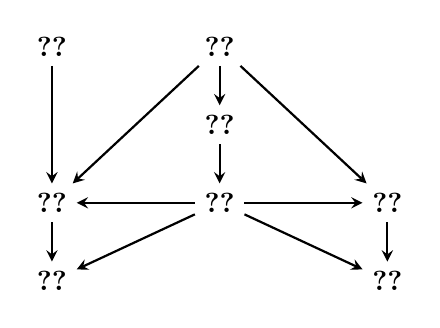
\begin{tikzpicture}[node distance=0.5cm and 1.5cm]
\node (E0) [] {\cref{prop0}};
\node (E1) [right=of E0] {\cref{prop1}};
\node (E2) [below=of E1] {\cref{prop2}};
\node (E3) [below=of E2] {\cref{prop3}};
\node (E4) [left=of E3] {\cref{prop4}};
\node (E5) [right=of E3] {\cref{prop5}};
\node (G1) [below=of E4] {\cref{eq:subtree}};
\node (G2) [below=of E5] {\cref{eq:distance}};

\draw[arrow] (E0) -- (E4);
\draw[arrow] (E1) -- (E4);
\draw[arrow] (E1) -- (E2);
\draw[arrow] (E1) -- (E5);
\draw[arrow] (E2) -- (E3);
\draw[arrow] (E3) -- (E4);
\draw[arrow] (E3) -- (E5);
\draw[arrow] (E3) -- (G1);
\draw[arrow] (E3) -- (G2);
\draw[arrow] (E4) -- (G1);
\draw[arrow] (E5) -- (G2);
\end{tikzpicture}
\caption{So bauen die Eigenschaften aufeinander auf.}
\end{figure}

\newpage
\begin{property}\label{prop0}
Für den Algorithmus gilt: \\
Wenn $\lambda_h = d_h$, dann gibt es entweder kein $j \in J$ mit $a_{hj} = 1$ oder es gibt ein $j \in J$ mit~$a_{hj} = 1$ und $\alpha(j) \geq h$.
\end{property}
\begin{proof}
Wenn $\lambda_h = d_h$ gesetzt wird, wurde zuvor keine Location hinzugefügt, da somit gilt, dass~$\hat{c}_j~=~0~<~d_h$ ist. Wird also eine Location $j$ hinzugefügt, muss $\hat{c}_j = d_h$ gelten, oder die Location wird erst später hinzugefügt. Somit muss $\alpha(j) \geq h$ sein.
\end{proof}

Die nächste Eigenschaft sagt aus, dass der lexikographisch kleinere Subtree nicht vor dem Anderen versorgt wird, wenn eine Location in beiden Subtrees vorkommt und noch zu bearbeiten ist.

\begin{property}\label{prop1}
Für den Algorithmus gilt: 
\[a_{hj} = a_{lj}  =1 \text{ mit } h<l \text{ und } j \in \hat{S} \text{ impliziert, dass } b_h(\hat{S}) \geq b_l(\hat{S})\]
\end{property}
\begin{proof}
Am Anfang des Algorithmus ist diese Eigenschaft wahr, da $b_h \geq b_l$ für $h<l$, weil~$b$ nur aus Einsen besteht. Im späteren Verlauf kann dies nur verletzt werden, wenn für Zeile~$h$ zuerst eine Location eröffnet wird. Dann gilt: \[b_h(\hat{S}) = b_h - \sum_{j \in S\setminus \hat{S}} a_{hj}x_j = 0 < 1 = b_l(\hat{S})\] 
Das ist nur möglich, wenn zu einem Zeitpunkt für die letzte Spalte $k$ in $\hat{S}$ gilt: $a_{hk} = 1$ und~$a_{lk} = 0$. Dies ist ausgeschlossen, da $A$ in \textit{standard greedy form} ist. \end{proof}

Als nächstes wird festgehalten, dass in jedem Schritt des Algorithmus nicht mehr Facilities in einem Subtree eröffnet werden können, als ihn versorgen können. Im Falle des \textit{UFLP} auf Bäumen also nur eine.

\begin{property}\label{prop2}
Für den Algorithmus gilt: \[b_h(\hat{S}) \geq 0 \quad \forall h \in Z\]
\end{property}
\begin{proof}
Dies ist wiederum am Anfang des Algorithmus wahr, da $b_h = 1$ für alle $h~\in~\{1,\dots, n^*\}$. Im Verlauf des Algorithmus ist durch \cref{prop1} gegeben, dass $b_h(\hat{S}) < 0$ nur auftritt, wenn der~$h$-te Subtree schon versorgt wird und zusätzlich eine Facility darin eröffnet wird. Dies entspricht~$h>~\alpha(k)$ und $a_{hk} = 1$, was durch die Definition von $\alpha(k)$ als größtem Index~$i$ mit $\lambda_i > 0$ und $a_{ik} = 1$ ausgeschlossen ist.
\end{proof}

\noindent Durch \cref{prop3} ist zu erkennen, dass, sollte die Menge $\hat{S}$ leer sein, alle Subtrees eine eröffnete Facility enthalten müssen.

\begin{property}\label{prop3}
Für den Algorithmus gilt: \[b_h(\emptyset) = 0 \quad \forall h \in Z\]
Das bedeutet, dass wenn alle Locations, beziehungsweise Spalten, in $S$ entweder eröffnet oder entfernt wurden, alle Subtrees in $Z$ versorgt werden.
\end{property}
\begin{proof}
Sei $h \in Z$. Dann muss ein $j \in S$ existieren mit $\alpha(j)=h$. In dem Schritt, in welchem~$j$ die letzte Spalte von $\hat{S}$ ist, wird $x_j = b_h(\hat{S})$ gesetzt und somit gilt nach diesem Vorgang~$b_h(\hat{S}) = 0$ und in Kombination mit \cref{prop2} gilt $b_h(\emptyset) = 0$.
\end{proof}

Außerdem gilt, sollte in Schritt $h$ noch kein Standort aus dem entsprechenden Subtree zu~$S$ hinzugefügt worden sein und auch in diesem Schritt keiner hinzugefügt werden, kann die Anzahl der eröffneten Facilities in diesem Subtree nicht größer als $b_h = 1$ werden.

\begin{property}\label{prop4}
Für den Algorithmus gilt: \[\lambda_h > 0 \text{ und } h \notin Z \text{ implizieren, dass } \sum_{j \in J} a_{hj}x_j \leq b_h \text{ gilt.}\]
\end{property}
\begin{proof}
Wenn $\lambda_h > 0$ und $h \notin Z$, gibt es nach \cref{prop0} zwei Möglichkeiten: \\

\noindent \textbf{1.} Es gibt kein $j \in J$, sodass $a_{hj} = 1$. Dann gilt $\sum_{j \in J} a_{hj}x_j = 0 \leq 1 = b_h$. \\

\noindent \textbf{2.} Es gibt ein $j \in J$ mit $a_{hj} = 1$ und $\alpha(j) > h$. Dann gilt nach \cref{prop1} und \cref{prop3}:~$b_h(\emptyset) \geq b_{\alpha(j)}(\emptyset) = 0$. Somit muss $b_h = 1 \geq 1 = \sum_{j \in J} a_{hj}x_j$ sein.
\end{proof}

Besonders intuitiv für das \textit{UFLP} auf Bäumen ist die folgende Eigenschaft, nach der gilt, dass wenn bereits ein Standort aus dem $h$-ten Subtree zu $S$ hinzugefügt wurde, dieser in der Lösung auf jeden Fall eine eröffnete Facility enthält.

\begin{property}\label{prop5}
Für den Algorithmus gilt: \[ \text{Wenn } \lambda_h = 0 \text{, dann ist: } \sum_{j \in S} a_{hj}x_j \geq b_h\text{.}\]
\end{property}
\begin{proof}
Wenn $\lambda_h = 0$ ist, muss in einem vorangegangenen Schritt bereits ein $j \in J$ zu $S$ hinzugefügt worden sein, für welches $a_{hj} = 1$ gilt. Also existiert ein $j\in S$ mit $a_{hj} = 1$ und~$\alpha(j) < h$. Nach \cref{prop1} und \cref{prop3} gilt $b_h(\emptyset) \geq b_{\alpha(j)}(\emptyset) = 0$. \\
Daraus folgt: \[\sum_{j \in S} a_{hj}x_j = 1 \geq 1 =~b_h\]
\end{proof}

Nun folgt mithilfe der festgestellten \cref{prop0,prop1,prop2,prop3,prop4,prop5} der Beweis dafür, dass für den Algorithmus von Hoffman et al. auch die \cref{eq:subtree,eq:distance} gelten.

\begin{lemma}
Die \cref{eq:subtree} gilt für den Algorithmus von Hoffman et al.
\end{lemma}
\begin{proof}
Da von $\lambda_h$ und $\sum_{j \in J} a_{hj}x_j + z_h - b_h$ mindestens eines der Zahl $0$ entsprechen muss, wird überprüft, was passiert, wenn dies bei einem nicht der Fall ist. \\
Sei $\lambda_h > 0$. Dann gibt es zwei mögliche Fälle: \\

\noindent \textbf{1.} Sei $h \in Z$: Dann gilt nach \cref{prop3}, dass $b_h(\emptyset) = 0$ sein muss und somit $\sum_{j \in S} a_{hj}x_j =~1$, da nach Problemstellung $b_h = 1$ ist. Da im Algorithmus $x_j = 0$ für alle $j \notin S$ gesetzt wird, gilt auch~$\sum_{j \in J}a_{hj}x_j = 1$ und somit $z_h = 0$. Daraus folgt: 
\[\sum_{j \in J} a_{hj}x_j + z_h - b_h = 1 + 0 - 1 = 0\]

\noindent \textbf{2.} Sei $h \notin Z$: Dann gilt nach \cref{prop4}: $\sum_{j \in J} a_{hj}x_j \leq b_h$. 
Da $b_h = 1$ ist lässt sich das Zusammenspiel aus $z_h$ und der Summe nutzen. 
Ist $z_h = 0$, gibt es einen Knoten $j$ mit~$a_{hj} = 1$ und~$x_j = 1$ und daher muss $\sum_{j \in J} a_{hj}x_j > 0$ sein. 
Also $\sum_{j \in J} a_{hj}x_j = 1$ und somit \[\sum_{j \in J} a_{hj}x_j + z_h - b_h = 1 + 0 - 1 = 0.\]
Ist $z_h = 1$, dann ist $\sum_{j \in J} a_{hj}x_j = 0$ und somit \[\sum_{j \in J} a_{hj}x_j + z_h - b_h = 0 + 1 -1 = 0.\] 
Analog lässt sich sagen, dass wenn $\sum_{j \in J} a_{hj}x_j + z_h - b_h \neq 0$ ist, $\sum_{j \in J} a_{hj}x_j > 1$ sein muss. Das würde bedeuten, dass $\sum_{j \in J} a_{hj}x_j > b_h$ ist, was für $h \in Z$ gegen \cref{prop3} verstoßen würde, weil dann~$b_h(\emptyset) < 0$ wäre. Es muss also $h \notin Z$ sein. \\
Da nach \cref{prop4} bei~$\lambda >~0$ dann~$\sum_{j \in J} a_{hj}x_j \leq b_h$ wäre, was ein Widerspruch zu den bisherigen Folgerungen wäre, muss außerdem~$\lambda_h = 0$ sein. \end{proof}

\begin{lemma} \cref{eq:distance} gilt für den Algorithmus von Hoffman et al. \end{lemma}
\begin{proof}Da mindestens ein Term von $z_h$ und $\lambda_h-d_h$ dem Wert $0$ entsprechen muss, wird überprüft was passiert, wenn einer von beiden ungleich $0$ ist. Sollte $\lambda_h-d_h \neq 0$ sein, gibt es mehrere Möglichkeiten wie dies zustande kommt. \\

\noindent \textbf{1.} Sei $\lambda_h = 0$: Da $d_h \neq 0$ sein muss aufgrund seiner Definition, führt dies zu $\lambda_h-d_h < 0$. Durch \cref{prop5} gilt wenn $\lambda_h = 0$, dann $\sum_{j \in J} a_{hj}x_j \geq b_h$. Da somit in $h$-ten Subtree eine Facility eröffnet wird, gilt $z_h = 0$. \\

\noindent \textbf{2.} Sei $\lambda_h > 0, h \notin Z$: Hier lässt sich leicht erkennen, dass es kein $j \in J$ gibt mit $\alpha(j) = h$. Somit muss der Algorithmus im $h$-ten Schritt die Distanz $d_h$ ausgewählt haben und somit gilt $\lambda_h = d_h$ und $\lambda_h-d_h = 0$. \\

\noindent \textbf{3.} Sei $\lambda_h > 0, h \in Z$: Durch \cref{prop3} ist $b_h(\emptyset) = 0$ gegeben für ein $h \in Z$ wie es hier vorgefunden wird. Da $b_h = 1$, muss $\sum_{j \in J} a_{hj}x_j = 1 = b_h$ sein und dadurch gilt $z_h = 0$. \\

\noindent Angenommen, $z_h \neq 0$, dann ist $z_h = 1$ und es gibt kein $j \in J$ mit $a_{hj} = 1$ und $x_j = 1$. Somit ist~$b_h(\emptyset) > 0$, weshalb ausgeschlossen werden kann, dass $h \in Z$ ist. Da schon gezeigt wurde, dass bei~$\lambda_h = 0$, dann $z_h = 0$ folgt und bei~$\lambda_h > 0$ mit $h \notin Z$, dann $\lambda_h = d_h$ folgt, ist dieser Fall auch abgedeckt. \end{proof}

Mit \cref{prop2} lässt sich außerdem zeigen, dass $x_j \geq 0$ für alle $j \in S$ und somit die Lösung~$x,z$ gültig ist. 


\subsection{Komplexität}\label{sec:komp1}
Kolen schreibt in \cite{Kol83}, dass sein Algorithmus eine Laufzeit von $O(n^3)$ für das \textit{UFLP} auf Bäumen hat, wobei $n$ die Anzahl aller Knoten ist, also $n = |I \cup J|$. Die Berechnung setzt sich wie folgt zusammen: \\
Die Berechnung der Distanzen zwischen einem Knoten und allen Anderen und das Sortieren dieser benötigt $O(n \log n)$ Schritte. \\
Somit benötigt man für alle Subtrees eines Knotens $O(n \log n)$ Schritte.
Deshalb und weil es nur~$n^2$ Subtrees geben kann, benötigt das Finden aller Subtrees $O(n^2 \log n)$ Schritte. 
Nach \cite{Aho+74} kann eine lexikografisch nicht absteigende Ordnung für $n$ Mengen mit $m$ Elementen mithilfe von Radixsort in $O(nm)$ hergestellt werden. Bei bis zu $n^2$ Subtrees, die jeweils bis zu $n$ Einträge haben können, benötigt man also $O(n^3)$ Schritte. \\
Auch die duale Lösung wird mithilfe der $n^* \leq n^2$ Zeilen der Matrix berechnet und es werden pro Durchgang höchstens $n$ Locations zu $S$ hinzugefügt. Somit wird die duale Lösung in~$O(n^3)$ berechnet. \\
Die Alternative Berechnung, welche in \cref{sec:hoffmanetal} erwähnt wird, reduziert dies zu $O(n^2)$ \cite{KolTam90}. Dadurch könnte eine Instanz des \textit{UFLP} auf Bäumen, welche mit der Subtree-Matrix gegeben ist, mit diesem Algorithmus in $O(n^2)$ gelöst werden. \\
Der Teil des Algorithmus, der die primale Lösung berechnet, nutzt die~$|Z| \times |S|$ große Submatrix und behandelt jeden Eintrag höchstens einmal. Somit benötigt dieser Teil~$O(n^2)$ Schritte. Die Gesamtkomplexität beläuft sich somit auf $O(n^3)$. Somit hat der Algorithmus eine polynomielle Laufzeit.

\pagebreak
\section{Beweis von Cornuejols et al.}\label{sec:cornuejols}
\begin{wrapfigure}{r}{0.6\textwidth}\vspace*{-0.7cm}
\begin{definition}[\textit{Tree Partition Problem} $P_2$]\label{def:P2}
\[\text{Hier gilt: }y_{ij} = \begin{cases} 1 \quad v_i \text{ liegt im Subbaum von } v_j \\ 0 \quad \text{ sonst.}	
	\end{cases}\]
\begin{align*}
	\max & \sum_{i} \sum_{j} \gamma_{ij} y_{ij} && \\
	\text{unter } & \sum_{j} y_{ij} = 1 && \forall v_i \in V \\
	& y_{ij} - y_{i'j} \leq 0 && \forall v_i,v_{i'},v_j \in V \text{, wobei }v_{i'} \\
	&&& \text{ zwischen } v_i \text{ und } v_j \text{ liegt.} \\
	& y_{ij} \in \{0,1\} && \forall v_i,v_j \in V
\end{align*}

	\label{def:treepartition}
%$y_{ij} = 1$, wenn $v_i$ im Subbaum von $v_j$ liegt und $y_{ij} = 0$, sonst.
\end{definition}
\end{wrapfigure} 
Der Beweis von Cornuejols et al. wurde 1990 in \textit{Discrete Location Theory} \cite{MirFra90} veröffentlicht und beruht darauf, das Problem auf eine Variante von \textit{Tree Partition} zu reduzieren (\cref{sec:reduction}) und diese dann mit dem polynomiellen Algorithmus von Bárány et al. (\cite{Bar+86}) zu lösen (\cref{sec:barany}). Das \textit{Tree Partition} Problem besteht aus einem Baum mit Gewichten $\gamma_{ij}~\in~\Z$ für jede Kombination aus Knoten $v_i, v_j$ als Eingabe und der Anforderung, die Aufteilung des Baumes zu finden, die das maximale Gewicht hat. Dabei werden die Gewichte zwischen der Wurzel des Subbaumes und allen Knoten des Subbaumes summiert. \\

Für die Lösung wird die optimale Zugehörigkeit der Knoten zu den Subbäumen rekursiv berechnet. Der genaue Algorithmus wird in den folgenden Abschnitten erklärt \cite{Cor+90}. 

\subsection{Algorithmus}
Wie bereits erwähnt, besteht die Methode aus zwei Teilen: die Reduktion auf das \textit{Tree Partition Problem} und die Anwendung des Algorithmus von Bárány et al.. Diese Vorgänge werden in diesem Abschnitt beschrieben. 

\newpage
\subsubsection{Reduktion auf Tree Partition}\label{sec:reduction}
Für die Reduktion auf \textit{Tree Partition} werden Gewichte für alle Kombinationen von Knoten benötigt. 
\begin{wrapfigure}{r}{0.45\textwidth}\vspace*{-0.9cm}
\begin{definition}[Gewichte für \textit{Tree Partition}]
\[\gamma_{ij} = \begin{cases}
	-c_{j} \quad & i = j \land j \in J \\
	-M \quad & i = j \land j \notin J \\
	0 \quad & i \neq j \land i,j \notin I \\
	-t_{ij} \quad & \text{sonst}
	\end{cases}\]
\end{definition}
\end{wrapfigure}
\noindent Die Gewichte $\gamma_{ij}$ sind definiert, sodass, wenn~$i$ und $j$ zwei unterschiedliche Locations sind, das Gewicht $0$ entspricht. Das Gewicht $\gamma_{ii}$ entspricht den Standortkosten, falls $i$ eine Location ist und entspricht $M \in \Z$, wenn~$i$ ein Klient ist und keine mögliche Location.
Dabei ist $M$ eine sehr groß gewählte ganze Zahl.
Für alle anderen Fälle gilt:~$\gamma_{ij}$ entspricht den Transportkosten zwischen den beiden Knoten $v_i$ und $v_j$ \cite{Cor+90}. 

\noindent Da \textit{Tree Partition} ein Maximierungsproblem ist, \textit{UFLP} allerdings ein Minimierungsproblem, müssen die Gewichte mit $-1$ multipliziert werden.
Die Gewichte~$-t_{ij}$ werden offensichtlicherweise benutzt, um die Transportkosten zu minimieren. Dadurch, dass für die Wurzel $j$ eines Subbaumes auch das Gewicht $\gamma_{jj}$ in das Gesamtgewicht eingerechnet wird, können die Standortkosten ebenfalls berücksichtigt werden. Dadurch, dass für die Kanten von Klienten zu sich selbst ein Gewicht von $-M$ benutzt wird, wird ausgeschlossen, dass ein Klienten-Knoten zur Wurzel eines Subbaums wird.
Für zwei unterschiedliche Locations sind die Gewichte $0$, damit diese keine Auswirkungen auf die optimale Lösung haben, falls einer von ihnen nicht eröffnet wird \cite{Cor+90}. Sollten die Locations auch gleichzeitig Klienten sein, werden die normalen Transportkosten verwendet. \\

\begin{example}{Umwandlung der Kosten in Gewichte}{ex:weights}
Für das Beispiel aus~\Cref{ex:example} werden hier die Gewichte berechnet, wobei die Matrix entsprechend der alphabetischen Reihenfolge der Knoten sortiert ist:\\
\begin{minipage}[c]{0.45\textwidth}
\begin{tikzpicture}[node distance=2cm]
\node[client,label=north:$\textcolor{darkgray}{-M}$] (R) {$R$};
\node[location, below left of=R, label=315:$\textcolor{cyan}{-2}$] (B) {$B$};
\node[client, below right of=R, label=north east:$\textcolor{darkgray}{-M}$] (C) {$C$};
\node[client, below left of=B, label=east:$\textcolor{darkgray}{-M}$] (D) {$D$};
\node[location, below left of=C, label=east:$\textcolor{cyan}{-2}$] (E) {$E$};
\node[location, below right of=C, label=west:$\textcolor{cyan}{-2}$] (F) {$F$};

\draw[edge] (R) --node[above left] {$-3$} (B);
\draw[edge] (R) --node[above right] {$-2$} (C);
\draw[edge] (B) --node[above left] {$-1$} (D);
\draw[edge] (C) --node[above left] {$-1$} (E);
\draw[edge] (C) --node[above right] {$-2$} (F);
\end{tikzpicture}
\end{minipage} \begin{minipage}[c]{0.45\textwidth}
\[\gamma = 
\myvec{	-M & -3 & -2 & -4 & -3 & -4 \\ 
		-3 & -2 & -5 & -1 & 0 & 0 \\
		-2 & -5 & -M & -6 & -1 & -2 \\
		-4 & -1 & -6 & -M & -7 & -8 \\
		-3 & 0 & -1 & -7 & -2 & 0 \\ 
		-4 & 0 & -2 & -8 & 0 & -2}\]
\end{minipage}
\end{example}


\subsubsection{Tree Partition Algorithmus von Bárány et al.}\label{sec:barany}
Der polynomielle Algorithmus für \textit{Tree Partition} basiert auf zwei Rekursionsgleichungen. Außerdem wird eine Ordnung über die Wahl eines Wurzelknotens $r$ induziert. Diese funktioniert nur über die Kantenrelation und nicht über die Transportkosten wie beim Algorithmus von Kolen. Für den Beispielgraph würden, wenn man $A$ als Wurzel wählt, $B$ und $C$ darauf in keiner festen Reihenfolge folgen. Die Wurzel hilft außerdem dabei, zwei Mengen zu definieren, die in den Rekursionsgleichungen benötigt werden: \\ 

\noindent \begin{minipage}[c]{0.5\textwidth}
\begin{definition}[Induzierter Subbaum]
Sei $r \in V$ die Wurzel des Baumes. Der induzierte Subbaum von $v \in V$ ist: \\
\[V(v) = \{u \in V \mid v \in P(r,u)\}\]
\end{definition}
\end{minipage} \begin{minipage}[c]{0.5\textwidth}
\begin{definition}[Direkte Nachfolger]\label{def:successor}

Die direkten Nachfolger von $v \in V$ sind \\ definiert als: \\
\[S(v) = \{u \in V \mid u \in V(v) \land \{v,u\} \in E\}\]
\end{definition}
\end{minipage} \\

Der induzierte Subbaum eines Knotens $v$ ist also der Baum, der aus allen Nachfolgern von $v$ besteht. Aus dieser Menge lässt sich außerdem die Menge der direkten Nachfolger von~$v$ herauslösen, die aus allen jenen Knoten besteht, die in $V(v)$ sind und eine Kante zu~$v$ besitzen \cite{Bar+86}. 
 
\begin{wrapfigure}{r}{0.35\textwidth}\vspace*{-0.7cm}\begin{definition}[\\ Rekursionsgleichung 1]
\[g(v) = \underset{u \in V(v)}{\max} g_u(v)\]
\end{definition}\end{wrapfigure}
\noindent Auf den ausgewählten Wurzelknoten wird nun Rekursionsgleichung 1 angewandt.
Diese wählt das Maximum aus allen möglichen Berechnungen von Rekursionsgleichung 2 für $r$ aus. In Rekursionsgleichung 2 steht das $u$ für den Knoten, in dessen Subbaum $v$ liegt. Es wird also berechnet, in welchem Subbaum~$r$ das meiste Gewicht zur Summe hinzufügen kann beziehungsweise durch die Versorgung von welcher Facility die niedrigsten Kosten entstehen \cite{Bar+86}.

\begin{definition}[Rekursionsgleichung 2]
\[g_u(v) = \begin{cases} \gamma_{vu} + \sum_{w \in S(v)} \max\{g_u(w), g(w)\} \quad & u \notin V(v)\setminus \{v\} \\
				\gamma_{vu} + \sum_{w \in S(v)\setminus \{w^*\}} \max\{g_u(w), g(w)\} + g_u(w^*) \quad & u \in V(v)\setminus \{v\}
			\end{cases}\]
mit $w^* =$ Knoten zwischen $v$ und $u$.
\end{definition}

Es wird also für die Kombination aus Klientenknoten $v$ und Facility-Knoten $u$ die Summe der maximalen Gewichte der direkten Nachfolger von $v$ auf die Transportkosten von $u$ zu~$v$ addiert. Die Funktion~$\max\{g_u(w),g(w)\}$ berechnet die bessere Option aus $u$ versorgt~$w$ und~$w$ wird von einer Facility aus dem eigenen induzierten Subbaum versorgt \cite{Bar+86}. \\

Für die Blätter $b$ im Baum, also jene Knoten, die keine Nachfolger in der induzierten Ordnung haben gilt:
\[g(b) = g_b(b) = \gamma_{bb} \quad \text{ und } \quad g_u(b) = \gamma_{ub} \quad \text{\cite{Cor+90}}\]

\begin{example}{Rekursionsgleichungen: Blätter}{ex:recursionleafs}
	Für das Beispiel aus \Cref{ex:example} werden zunächst die Gewichte der Blätter berechnet: 
	\[ g(D) = g_D(D) = -M \quad g(E) = g_E(E) = -2 \quad g(F) = g_F(F) = -2 \]
		\[ g_B(D) = -1 \quad g_C(E) = -1 \quad g_C(F) = -2 \]
\end{example}


\begin{example}{Rekursionsgleichungen: Innere Knoten}{ex:recursion}
	Nun wird weiter in Richtung Wurzel gerechnet, also folgen die Knoten $B$ und $C$.
	Zu Zwecken der Übersichtlichkeit wird bei Auftreten des Wertes $-M$ die Berechnung des jeweiligen Pfades abgebrochen und nur die Berechnung für $C$ vollständig gezeigt. Ein abgebrochener Pfad wird mit dem Symbol $\blitz$ markiert.
	\begin{eqnarray*}
		g(B) &=& \max\{g_B(B), g_D(B)\} = -3 \\
		g(C) &=& \max\{g_C(C), g_E(C), g_F(C)\} \\
		&=& \max\{-M + ... \blitz , -1 + \max\{g_E(F),-2\} +g_E(E), -2 \\ && + \max\{g_F(E), -2\} +g_F(F) \} \\
		&=& \max\{-M\blitz , -1 +\max\{0, -2\} -2, -2 + \max\{0, -2\} -2\} \\
		&=& \max\{-M \blitz , -3, -4\} = -3  
	\end{eqnarray*}
\end{example}
\begin{example}{Rekursionsgleichungen: Wurzel}{ex:recursionroot}
	Für die Wurzel wird aus Platzgründen nur die Berechnung von $g_B(R)$ vollständig gezeigt:
	\begin{eqnarray*}
		g_R(R) &=& g_C(R) = g_D(R) = -M \blitz  \\
		g_B(R) &=& -3 + \max\{g_B(C),g(C) = -3\} + g_B(B)  \\
		&=& -3 + \max\{-5 + \max\{g_B(E) = 0, g(E) = -2\} \\
		&& + \max\{g_B(F) = 0, g(F) = -2\}, -3\} -3 \\
		&=& -3 + \max\{-5, -3\} -3 = -9 \\
		g_E(R) &=& -9 \\
		g_F(R) &=& -10		
	\end{eqnarray*}
	\begin{eqnarray*}
		g(R) &=& \max \{g_R(R), g_B(R), g_C(R), g_D(R),g_E(R), g_F(R)\} \\
		&=& \max\{-M, \textbf{-9}, -M, -M, \textbf{-9}, -10\} = -9 
	\end{eqnarray*}		
	Daraus lässt sich schließen, dass $R$ entweder von $B$ oder von $E$ versorgt werden sollte.
\end{example}

Aus dem maximalen Gewicht, welches negativ ist, lassen sich durch Multiplikation mit~$-1$ die minimalen Kosten berechnen. Wie man im Beispiel sehen kann, wird durch die Auswahl des maximalen Terms aus $\{g_u(v) \mid u \in V(v)\}$ ersichtlich, von welcher Facility der Knoten~$v$ versorgt wird. Die gesamte Zuordnung kann aus der Berechnung der optimalen Kosten interpretiert werden. Bei einer Unterscheidung zwischen $g_u(v)$ und $g(v)$ steht, wie bereits erwähnt,~$g_u(v)$ dafür, dass $v$ von $u$ versorgt wird und $g(v)$ dafür, dass $v$ von einem Location-Knoten aus $V(v)$ versorgt wird. \\

Um die Berechnung zu vereinfachen und zur Verbesserung der Laufzeit können die berechneten Werte für $g_u(v)$ und $g(v)$ abgespeichert werden.

\subsection{Korrektheit}\label{sec:korrektheit2}
Die Reduktion auf \textit{Tree Partition} wird in \cite{Cor+90} beschrieben und lässt sich ebenso überprüfen, wie der Beweis für \textit{Tree Partition} in \cite{Bar+86}. Dafür wird für den Algorithmus die Gültigkeit und die Optimalität der generierten Lösung überprüft.

\newpage
\subsubsection{Reduktion auf \textit{Tree Partition}}
Die Reduktion auf \textit{Tree Partition} ist in \cite{Cor+90} beschrieben und funktioniert über eine Umformung der Nebenbedingungen und einer Zusammenführung der Kosten in eine einzige Gewichtsfunktion. Die Umformung des LPs ist hier nachvollziehbar aufgezeigt: \\

\noindent \begin{minipage}[c]{0.47\textwidth}\vspace*{-0.7cm}
\begin{defi}{Ursprüngliches LP}
\begin{eqnarray*}
\min & \sum_{i\in I} \sum_{j \in J} t_{ij}y_{ij} &+ \sum_{j\in J} c_jx_j  \\
\text{unter} & \sum_{j \in J} y_{ij} = 1 & \forall i \in I \\
& y_{ij} \leq x_j & \forall i \in I, j\in J \\
& x_j, y_{ij} \in \{0,1\} & \forall i\in I, j\in J
\end{eqnarray*}
\end{defi}
\end{minipage} \begin{minipage}[c]{0.03\textwidth}
\hfill
\end{minipage} \begin{minipage}[c]{0.5\textwidth}
Die Schritte, die in \cite{Cor+90} beschrieben werden, sind die Umwandlung der Kosten $t_{ij}$ und $c_j$ zu Gewichten $\gamma_{ij}$, das Zusammenfassen der Entscheidungsvariablen $x$ und $y$ zu einer einzigen und implizit die Umwandlung zu einem Maximierungsproblem. \\

Die Zielfunktion wird durch das Ersetzen der Kosten und der Umwandlung in ein Maximierungsproblem zu: 
\end{minipage} \\

\[\max \sum_{i\in I} \sum_{j \in J} \gamma_{ij}y_{ij} + \sum_{j \in J} \gamma_{jj}x_j\]

\noindent Und durch das Zusammenfassen der Entscheidungsvariablen erhält man diese Zielfunktion:
\[\max \sum_{i\in I} \sum_{j \in J} \gamma_{ij}y_{ij} + \sum_{j \in J} \gamma_{jj}y_{jj}\]

Es ist möglich die Entscheidungsvariablen zusammenzufassen, da zuvor keine Werte für~$y_{jj}$ definiert waren, weil es keine Schleifen im Graphen geben kann. Dadurch, dass für $\gamma_{ii}$ mit~$i~\notin~J$ Werte benutzt werden, die vom Algorithmus nie ausgewählt werden und $\gamma_{ij} = 0$ für~$i,j \in J$, können keine unzulässigen Lösungen berechnet werden. Durch ersteres wird nie ein Klientenknoten als Facility ausgewählt und durch die zweite Vorkehrung wird verhindert, dass Knoten versorgt werden, obwohl sie keinen Klienten entsprechen. Da in \textit{Tree Partition} die Klienten und Locations als gleichwertig betrachtet werden, benutzen wir die Notation $K$ für $I \cup J$, also die Menge aller Knoten. \\
Die Zielfunktion kann nun noch einmal umgeformt werden zu:
\[\max \sum_{i\in K} \sum_{j \in K} \gamma_{ij}y_{ij}\]

\newpage

Die Nebenbedingungen sind durch den Schritt der Zusammenfassung der Entscheidungsvariablen ebenfalls verändert worden: \\
\[\sum_{j \in J} y_{ij} = 1 \quad \forall i \in I \text{ wird zu } \sum_{j \in I \cup J} y_{ij} = 1 \quad \forall i \in K\]

\[x_j, y_{ij} \in \{0,1\} \quad \forall i\in I, j\in J \text{ wird natürlich zu } y_{ij} \in \{0,1\} \quad \forall i,j \in K\]

\[y_{ij} \leq x_j \quad \forall i \in I, j\in J \text{ wird zu }  y_{ij} \leq y_{jj} \quad \forall i,j \in K\]

Nun lässt sich die letzte Bedingung noch etwas umformen: \\
\[ y_{ij} \leq y_{jj} \quad \forall i,j \in K \Leftrightarrow  y_{ij} - y_{jj} \leq 0 \quad \forall i,j \in K \]
Diese Bedingung sorgt dafür, dass ein Knoten nur einem Subbaum zugeordnet werden kann, dessen Wurzel ebenso diesem Subbaum zugeordnet ist. Entsprechend für das \textit{UFLP} auf Bäumen wäre das: Ein Klient kann nur einer eröffneten Location zugeordnet werden. Diese Bedingung kann auf alle Knoten zwischen $i$ und $j$ ausgeweitet werden. Da es nur einen Pfad zwischen $i$ und $j$ gibt, gilt, wenn Klient $i$ Location $j$ zugeordnet wird, dass für alle Knoten vor~$v_i$ auf diesem Pfad, $j$ die günstigste Location ist. Diese Aussage wird in \cite{Cor+90} bewiesen: 

\begin{proof} Angenommen,$i$ wird weiterhin von $j$ versorgt und $i'$ würde nicht von $j$ versorgt werden, sondern von $j' \neq j$. Dann wären die Kosten dieser Versorgung $t_{i'j'} + c_{j'} + t_{ij} + c_j$. Die Alternative, in der beide Klienten von $j$ versorgt werden, hat die Kosten $t_{ij} + c_j + t_{i'j} + c_{j'}$.
Laut der Annahme müsste $t_{i'j'} + c_{j'} + t_{ij} + c_j \leq t_{ij} + c_j + t_{i'j} + c_{j'}$ gelten und somit $t_{i'j'} \leq t_{i'j}$.
Da es nur einen Pfad zwischen $v_{i'}$ und $v_i$ geben kann, muss damit gelten, dass $t_{ij'} \leq t_{ij}$ ist. Somit ist die Annahme nicht optimal und für alle Knoten $v_{i'}$ auf dem Pfad zwischen $v_i$ und~$v_j$ gilt: Wird $i$ von $j$ versorgt, muss auch $i'$ von $j$ versorgt werden. \end{proof}

Es wird also in jedem Fall ein Subbaum gebildet, der einem Wurzelknoten zugehörig ist. Also kann die Nebenbedingung formuliert werden als:
\[y_{ij} - y_{i'j} \leq 0 \quad \forall i,i',j \in K \text{, wobei } v_{i'} \text{ vor } v_i \text{ auf dem Pfad von } v_j \text{ zu } v_i \text{ liegt.}\]

\noindent Somit wurde das LP aus \cref{def:treepartition} aus dem Ursprungsproblem geformt. Somit muss auch jede Lösung für das Ursprungsproblem durch die Umformung zu einer Lösung von \textit{Tree Partition} werden.
\newpage
\subsubsection{Optimalität der Lösung}
Zu zeigen ist, dass $g(r) = \max\{g_v(r) \mid v \in K\}$ die optimale Lösung des umgeformten IP $\max \sum_{i \in K}\sum_{j \in K} \gamma_{ij}y_{ij}$ ist und somit die optimale Aufteilung der Knoten in Subbäume. \\
Dafür wird das duale LP aufgestellt und im Anschluss gezeigt, dass eine Lösung des dualen LPs, die gleich der Lösung des Algorithmus ist, gültig für das duale LP ist.
Daraus folgt dann, dass die Lösung für das primale Problem optimal sein muss \cite{Bar+86}. \\

In \cref{def:successor} wurde die Menge $S(v)$ als Nachfolger des Knotens $v$ definiert. Diese Definition ist in Abhängigkeit zum Wurzelknoten $r$ durch die Verwendung des induzierten Subbaums $V(v)$. Die folgende Definition handelt davon, wenn statt der Wurzel ein beliebiger Knoten $u$ gewählt wird.
\begin{definition}[Nachfolger relativ zu einem anderen Knoten]
Seien $v,u \in V$ Knoten im Baum. Die Nachfolger von $v$ relativ zu $u$ sind definiert als:
\[S_u(v) = \{w \in V \mid v \in P(u,w) \land \exists \{v,w\} \in E\}\]
Für die Nachfolger von $v$ relativ zu sich selbst gilt:
\[S_v(v) = \{w \in V \mid \{v,w\} \in E\}\]
\end{definition}
Diese Definition wird benötigt für das duale LP und eine weitere Rekursionsgleichung.
Um das duale LP zu lösen wird eine Belegung für den Vektor $\lambda$ gesucht, welcher in der Rekursionsgleichung bereits vorkommt, aber erst in \cref{def:D2} definiert wird.

\begin{definition}[Rekursionsgleichung $\sigma$]\label{def:rek3}
\[\sigma (j,i) = \max\{0, \gamma_{ji} - \lambda_i + \sum_{k \in S_j(i)} \sigma(j,k)\}\]
\end{definition}

%In \cite{Bar+86} wird diese Gleichung als Maximalwert der gegebenen Parameter definiert. Dadurch wird die Differenz zwischen dem Kantengewicht und der dualen Lösung für $i$ und alle Nachfolger von $i$ relativ zu $j$ und deren Nachfolger etc. berechnet. Bei nur positiven Werten wie in \cite{Bar+86} angenommen, würde dies dazu führen, dass $\sigma(j,i) > 0$ dann gilt, wenn die Kantengewichte größer als die dualen Lösungen wären. Bei nur negativen Werten wäre diese Differenz ebenfalls negativ und würde somit nicht erfasst werden. Stattdessen hätte $\sigma(j,i)$ einen Wert größer $0$, wenn \todo{stimmt das?}

\noindent Da nun alle Notationen geklärt sind, kann das duale LP aufgestellt werden. Damit ein duales LP aufgestellt werden kann, wird die Bedingung $y_{ij} \in \{0,1\} \quad \forall i,j \in K$ relaxiert zu $y_{ij} \geq 0 \quad \forall i,j \in K$. Da das primale LP (\cref{def:P2}) in dieser Arbeit mit den Nebenbedingungen $\sum_{j \in K}y_{ij} = 1 \quad \forall i \in K$ definiert wurde, entfallen die Nebenbedingungen~$\lambda_i \geq 0 \quad \forall i \in K$ im dualen LP. \\

\noindent \begin{minipage}{0.75\textwidth}
\begin{definition}[Duales LP $D_2$ nach \cite{Bar+86}]\label{def:D2}
Die Notation wurde dieser Arbeit angepasst.
\begin{align}
\min \quad & \sum_{i \in K} \lambda_i && \\
\text{unter} \quad & \lambda_i + \sigma(j,i) - \sum_{l \in S_j(i)}\sigma(j,l) &&\geq \gamma_{ji} \quad i,j \in K: i \neq j  \label{neb1}\\
& \lambda_j - \sum_{l \in S_j(j)} \sigma(j,l) &&\geq \gamma_{jj} \quad j \in K \label{neb2}\\
& \sigma(j,i) && \geq 0 \quad i,j \in K \label{neb3}
\end{align} 
\end{definition} 
\end{minipage} \begin{minipage}{0.02\textwidth}
\hfill
\end{minipage} \begin{minipage}{0.23\textwidth}
Um eine Lösung für $D_2$ zu erhalten, die gleich der Lösung von $P_2$ ist, werden die Rekursionsgleichungen aus dem Algorithmus angewendet. Man berechnet:
\[\lambda_i = g(i) - \sum_{j \in S(i)} g(j)\]
\end{minipage} \\

\noindent Damit erhält man den Anteil, den jeder Knoten an den Gesamtkosten beziehungsweise dem Gesamtgewicht hat. \\
In \Cref{ex:lambda} wird gezeigt, wie diese Berechnung beim Beispielgraphen aussehen würde.

\begin{example}{Duale Lösung berechnen}{ex:lambda}
Für den Graphen aus \Cref{ex:example} gilt, wie in \Cref{ex:recursionleafs}, \Cref{ex:recursion} und \Cref{ex:recursionroot} festgetellt:
\[g(R) = -9, \quad g(B) = -3, \quad g(C)= -3\]
Somit wäre $\lambda_R = -9 - (-3) - (-3) = -3$ der Anteil den $R$ am Gesamtgewicht hat, nämlich das Gewicht $\gamma_{RB}$ bzw. $\gamma_{RE}$ oder für das Ursprungsproblem formuliert, die Transportkosten zur Facility die $R$ versorgt. \\
Nach dem gleichen Prinzip lassen sich
\[\lambda_B = M-3,\quad \lambda_C = -3,\quad \lambda_D = -M,\quad \lambda_E = \lambda_F = 0\]
berechnen.
\end{example}

\noindent Somit hätten $P_2$ und $D_2$ die gleiche Lösung. Um zu zeigen, dass diese Lösung gültig ist, wird nun geprüft, ob die \cref{neb1,neb2,neb3} von $D_2$ erfüllt werden.
Die \cref{neb3} gilt offensichtlicherweise allein durch die \cref{def:rek3} von $\sigma$. 

\begin{lemma} Es gilt \cref{neb1} durch die \cref{def:rek3} von $\sigma$. \end{lemma}
\newpage
\begin{proof}
Für \cref{neb1} gibt es zwei mögliche Fälle, die zu beweisen sind. \\
\textbf{Fall 1:} $\sigma(j,i) = \gamma_{ji} - \lambda_i + \sum_{l \in S_j(i)} \sigma(j,l)$: 
\begin{eqnarray*}
&& \lambda_i + \sigma(j,i) - \sum_{l \in S_j(i)} \sigma(j,l) \\
&=& \lambda_i + \gamma_{ji} - \lambda_i + \sum_{l \in S_j(i)} \sigma(j,l) - \sum_{l \in S_j(i)} \sigma(j,l) \\
&=& \gamma_{ji} \geq \gamma_{ji}
\end{eqnarray*}

\noindent \textbf{Fall 2:} $\sigma(j,i) = 0$ und somit $\gamma_{ji} - \lambda_i +\sum_{l \in S_j(i)} \sigma(j,l) < 0$:
\begin{eqnarray*}
&& \lambda_i + \sigma(j,i) - \sum_{l \in S_j(i)} \sigma(j,l) \geq \gamma_{ji} \\
&\Leftrightarrow& \lambda_i - \sum_{l \in S_j(i)} \sigma(j,l) \geq \gamma_{ji} \\
&\Leftrightarrow& \lambda_i \geq \gamma_{ji} + \sum_{l \in S_j(i)} \sigma(j,l) \\
\end{eqnarray*}
Die letzte Zeile gilt, da $\gamma_{ji} - \lambda_i +\sum_{l \in S_j(i)} \sigma(j,l) < 0$
\end{proof}

\noindent Nun gilt es noch zu zeigen, dass \cref{neb2} erfüllt wird. Dafür nutzt man:
 
\begin{property} \label{prop7} Sei $j \in V$: Es gilt $g(r(T) \geq \sum_{k \in T} \gamma_{jk} + \sum_{l \in S(T)} g(l)$ für den Algorithmus von Bárány et al. \end{property}
\begin{proof} Sei $r(T)$ die Wurzel des Subbaumes $T$ und $S(T)$ die Menge aller Nachfolger der Knoten in $T$ ohne $T$ selbst, also $S(T) = \bigcup_{u \in T} S(u) \setminus T$. 
\begin{eqnarray*}
g(r(T)) &=& \max\{g_k(r(T)) \mid k \in V(r(T))\} \\
&=& \max\{g_k(r(T)) \mid k \in T \cup \bigcup_{l\in S(T)} V(l)\} \\
&=& \max\{g_k(r(T)) \mid k \in T\} + \sum_{h \in \cup_{l \in S(T)} V(l)}\max \{g_u(l) \mid u \in V(l)\} \\
&=& \max\{g_k(r(T)) \mid k \in T\} + \sum_{l \in S(T)} g(l) 
\end{eqnarray*}
Da im Algorithmus für $g_k(i)$ immer das Maximum der Gewichte ausgewählt wird, kann dieser Wert nicht kleiner sein als die Summe aller Kantengewichte zwischen den Knoten in $T$ und~$j$. Somit gilt: \[\max\{g_k(r(T)) \mid k \in T\} \leq \sum_{k \in T} \gamma_{jk}\]
\end{proof}


\begin{lemma} Die Gleichung $\lambda_j - \sum_{l \in S_j(j)} \sigma(j,l) \geq \gamma_{jj} \quad \forall j \in K$ gilt für den Algorithmus von Bárány et al. \end{lemma}

\begin{proof}
\Cref{neb2} lässt sich umformen zu 
\[\gamma_{ji} - \lambda_j + \sum_{l \in S_j(j)} \sigma(j,l) \leq 0\]
und diese Aussage soll nun gezeigt werden.
Zu diesem Zweck wird für jeden Knoten $l \in V$ der größte Subtree $T \subseteq \{j\} \cup \{i \in V \mid \sigma(j,i) >0\}$ der $l$ enthält genutzt.
Daher gilt:
\begin{eqnarray*}
\gamma_{ji} - \lambda_j + \sum_{l \in S_j(j)} \sigma(j,l) &=& \gamma_{ji} - \lambda_j + \sum_{l \in S_j(j)} \gamma_{jl} - \lambda_{i} + \sum_{h \in S_j(l)} \gamma_{jh} - \lambda_h \dots \\ 
&=& \gamma_{ji} - \lambda_j + \sum_{k \in T\setminus\{j\}} \gamma_{jk} - \lambda_{k} \\
&=& \sum_{k \in T} (\gamma_{jk}-\lambda_k) \\
&=& \sum_{k \in T} \gamma_{jk} - \sum_{k \in T}\lambda_k \\
&=& \sum_{k \in T} \gamma_{jk} - (g(r(T) - \sum_{l \in S(T)} g(l))) \quad \mid \cref{prop7} \\
&\leq & 0
\end{eqnarray*}
\end{proof}
 Somit sind alle Nebenbedingungen erfüllt und $\lambda_i = g(i) - \sum_{j \in S(i)} g(j)$ ist eine gültige Lösung für $D_2$. Durch den Satz der starken Dualität (\cref{thm:strongduality}) muss also $y_{ij}$ mit $i,j \in K$ für $P_2$ die optimale Lösung sein.


\subsection{Komplexität}
Für einen Baum mit $n$ Knoten benötigt die Umformung des IPs $O(n^2)$ Schritte.
Die Bestimmung der $n^2$ Werte $\gamma_{ij} \quad \forall i,j \in K$ benötigt konstant viele Schritte, da lediglich überprüft werden muss welchen Status $i$ und $j$ haben. Die Werte müssen nicht errechnet werden, da sie gegeben sind. \\
Die Berechnung des optimalen Gewichts mithilfe des Algorithmus von Bárány et al. benötigt~$O(n^2)$ Schritte, da für jede Kombination der Knoten $v_i,v_j \in V$ der Wert $g_{v_i}(v_j)$ berechnet werden muss. Damit diese Werte nicht jedes Mal neu berechnet werden müssen, können sie gespeichert werden. Das Ermitteln von $g(v)$ für jeden Knoten $v \in V$ ist ebenfalls in $O(n^2)$ Schritten möglich, da das Maximum von höchstens $n$ Werten ermittelt werden muss.

\pagebreak

\section{Kontext}\label{sec:kontext}
Es gilt nun, die Algorithmen in ihren Kontext einzuordnen.
Der Beweis von Antoon Kolen stellt einen der ersten Algorithmen dar, der das \textit{UFLP} auf Bäumen in polynomieller Zeit gelöst hat und wird in einigen Publikationen (\cite{LowWen11,Cor+90,BilCos94} etc.) zitiert als der Beweis für die polynomielle Lösbarkeit des \textit{UFLP} auf Bäumen. \\
Der Algorithmus von Cornuejols et al. stellt eine Laufzeit-technische Verbesserung im Vergleich zum Algorithmus von Kolen dar. Später wurde von \cite{ShaFar01} ein weiterer Algorithmus entwickelt, der eine Laufzeit in $O(n \log n)$ besitzt und dafür ausnutzt, dass sich eine Instanz des \textit{UFLP} auf Bäumen in eine äquivalente Instanz auf einem Binärbaum umwandeln lässt \cite{ShaFar01}.
Wie dieser nutzt der Algorithmus aus \cite{Cor+90} eine Rekursionsgleichung und dynamische Programmierung. Dieser Ansatz wird auch von \cite{BilCos94} verwendet, wobei der Algorithmus dem von Cornuejols et al. sehr ähnlich ist. Der Unterschied liegt hauptsächlich darin, dass das Problem nicht zunächst auf \textit{Tree Partition} reduziert wird, sondern die Rekursionsgleichung direkt auf die Kosten angewendet wird. 
Im weiteren Verlauf dieses Kapitels werden andere polynomiell lösbare Versionen des \textit{UFLP} und ähnlicher Probleme vorgestellt. 

\subsection{Andere polynomiell lösbare Versionen des \textit{UFLP}}
Wie bereits erwähnt, ist das \textit{UFLP} $\mathcal{NP}$-schwer und somit wahrscheinlich nicht polynomiell lösbar. Es gibt allerdings weitere polynomiell lösbare Fälle. Das \textit{Economic Lot Size} Problem aus \cite{KraBil77}, die von \cite{Jon+95} definierte Form und Serienparallele Graphen \cite{HasTam86}.

\subsubsection{Economic Lot Size}\label{sec:els}
Krarup und Bilde bestimmen in \cite{KraBil77} eine Version des \textit{UFLP}, die durch Erfüllung einiger Bedingungen dem \textit{Economic Lot Size} Problem (\textit{ELSP}) entspricht.
Hier wird nun zunächst erläutert welche Bedingungen erfüllt werden müssen, bevor das \textit{ELSP} mit seiner Interpretation beschrieben wird. \\
Das Problem basiert auf einer Version des \textit{UFLP}, bei der durch die Facilities eine Nachfrage bei den Klienten bedient werden muss, und somit ein Klient auch von mehreren Facilities anteilig versorgt werden kann. Somit ist dieses Problem nicht als Ganzzahliges LP zu lösen. \\
Die Menge der Klienten muss dann noch so geordnet werden, dass die Matrix der Transportkosten $T = t_{ji} \in \R^{m\times n}, i\in I, j \in J$ die \cref{prop61,prop62} erfüllt.

\begin{property}\label{prop61} Diese beiden Punkte müssen erfüllt sein.
\begin{itemize}
\item Die Teilmenge der endlichen Elemente $t_{ij} < \infty$ in jeder Reihe müssen alle in benachbarten Spalten stehen.
\item Jede Spalte muss mindestens ein endliches Element enthalten
\end{itemize}
\end{property}

\begin{property}\label{prop62} Sei $v_i$ das letzte endliche Element in Reihe $i$. 
Für alle $i,p \in I$ \\ und $j \in \{k \in I \mid~t_{t_{ik} < \infty}\} \cap \{k \in I \mid t_{pk} < \infty\}$ gilt: \\
\[\text{Entweder } t_{ij} \leq t_{pj} \text{ und } v_i \geq v_p \text{ oder } t_{ij} \geq t_{pj} \text{ und } v_i \leq v_p.\]
\end{property}


\noindent Das \textit{ELSP} ist ein Problem, in welchem geplant werden soll, wann idealerweise Produkte hergestellt werden, die in bestimmten Zeiträumen verkauft werden. \\

\begin{wrapfigure}{l}{0.55\textwidth}\vspace*{-1cm}
\begin{definition}[\textit{Economic Lot Size} nach \cite{KraBil77}]
Das Problem wird als IP folgendermaßen geschrieben:
\begin{align*}
\min & \sum_{j = 1}^n (k_jx_j + \sum_{i=1}^n t_{ij}y_{ij}) &&  \\
\text{unter } & \sum_{j=1}^n y_{ij} \geq 1 \quad && \forall j \in I \\
& x_j - y_{ij} \geq 0 \quad && \forall i,j \in I \\
& y_{ij} \geq 0 \quad && \forall i,j \in I \\
& x_j \in \{0,1\} \quad && \forall j \in I 
\end{align*}
\end{definition} \end{wrapfigure}

Es gibt eine Menge an Monaten~$I$, wobei in jedem Monat eine bestimmte Anzahl $d_i \in \N$, $i \in~I$ an Produkten benötigt wird. Dies nennt sich die Nachfrage. Außerdem kann jeden Monat $j \in I$ eine Produktion angelegt werden, die bestimmte Einrichtungskosten $k_j \in \N$ und Produktionskosten per Produkteinheit~$p_j \in~\N$ hat. Außerdem gibt es Kosten $r_j \in \N$ dafür, die Produkte bis zum nachfolgenden Monat zu lagern. \\
Die Kosten zwischen den Monaten werden wie folgt definiert: \\
\[t_{ij} = \begin{cases} d_i(p_j + \sum_{t=1}^{i-1} r_t) & \text{für }j < i,\quad i,j \in I \\
d_ip_i & \text{für }i=j \quad i,j \in I \\
					\infty & \text{für } j > i, \quad i,j \in I \end{cases}\]
Die Variablen $x_j$ und $y_j$ sind dann wie folgt definiert:
\[x_j = \begin{cases} 1 & \text{in Monat }j\text{ wird produziert.} \\
				0 & \text{in Monat }j\text{ wird nicht produziert.}
\end{cases}\]
\[y_{ij} = \text{Anteil der Nachfrage aus Monat }i\text{, der durch die Produktion in Monat }j\text{ gedeckt wird.}\]

\noindent In \cite{KraBil77} wird ein $O(mn)$ Algorithmus für das angepasste \textit{UFLP} gegeben und die Korrektheit bewiesen. 


\subsubsection{Die Formulierung von Jones et al.}\label{sec:jones}
In \cite{Jon+95} wird eine weitere Form des \textit{UFLP}s gegeben, die in polynomieller Zeit lösbar ist. Diese basiert auf den \cref{prop63,prop64,prop65}, welche voraussetzen, dass die Indizes der Klienten und Standorte geordnet sind. \\
Zunächst werden zwei Mengen definiert:
\begin{definition}[Erreichbare Klienten/Facilities]
Seien $i \in I$ ein Klient und $j \in J$ ein möglicher Facility Standort.
\[S(i) = \{j \in J \mid i \text{ kann von }j \text{ versorgt werden.}\}\]
\[D(j) = \{i \in I \mid j \text{ kann } i \text{ versorgen.}\}\]
Außerdem ist $f(i)$/$l(i)$ der kleinste/größte Index $i$ für den $i \in D(j)$ gilt.
\end{definition}

Nun können die Eigenschaften dieser Version des \textit{UFLP} definiert werden.

\begin{property}[Kontinuität]\label{prop63}
Für alle $j \in J$ und $i,k,l \in I$ mit $i < k < l$ gilt: \\
Wenn $i \in D(j)$ und $l \in D(j)$, dann gilt: $k \in D(j)$
\end{property}

\begin{property}[Abfallend]\label{prop64}
Für alle $1 \leq j < p \leq m \in J$ gilt: \\
\[f(j) \leq f(p) \text{ und } l(j) \leq l(p)\]
\end{property}

\begin{property}[Monotonie]\label{prop65}
Sei $i \in I$. Falls $j,p \in S(i)$ und $t_{ji} \leq t_{pi} \in S(i)$, dann gilt: 
\[t_{ji} \leq t_{kp} \text{ für alle }k \in I \text{ mit } j,p \in S(k)\]
\end{property}

Jones et al. zeigen in ihrer Abhandlung, dass diese Form des \textit{UFLP} für einige Probleme anwendbar ist. So lassen sich das \textit{Capacity Expansion} Problem aus \cite{Raj92}, das \textit{Discrete Lot Sizing} Problem aus \cite{WagWhi58}, das \textit{Tool Selection Problem} von \cite{Das+90}, ein \textit{Inventory} Problem, ein \textit{Stochastic Demand} Problem, sowie das \textit{Facility Location} Problem auf einer Linie mithilfe dieser Form und des dazugehörigen Algorithmus lösen \cite{Jon+95}.

\pagebreak

\subsubsection{Serien-parallele Graphen}\label{sec:spgraph}
Die nächste Form sind Serien-parallele Graphen, welche zunächst definiert werden.

\begin{definition}[Serien-parallele Graphen]
Ein Serien-paralleler Graph ist ein Multigraph, der rekursiv definiert werden kann durch die Serienverbindung oder Parallelverbindung zweier Serien-paralleler Graphen. \\
Der einfachste Serien-parallele Graph ist eine Kante zwischen einem Startknoten $s$ und einem Endknoten $t$. 

\begin{center}
$G:$\quad 
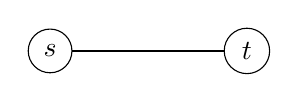
\begin{tikzpicture}[node distance = 2.5cm]
\node[white] (s) {$s$};
\node[white, right of=s] (t) {$t$};

\draw[edge] (s) -- (t);
\end{tikzpicture} \end{center}

Eine Serienverbindung aus den Graphen $G = (V=\{s,t\}, E =\{\{s,t\}\})$ und $G' = (V'=\{s',t'\}, E' = \{\{s',t'\}\})$ ist der Graph $S(G,G') = (V_s = \{s,u,t'\}, E_s = \{\{s,u\}\{u,t'\}\})$. \\
\begin{center}
$S(G,G'):$ \quad 
\begin{tikzpicture}[node distance = 2.5cm]
\node[white] (s) {$s$};
\node[white, right of=s] (u) {$u$};
\node[white, right of=t] (t'){$t'$};

\draw[edge] (s) -- (u);
\draw[edge] (u) -- (t');
\end{tikzpicture} \\ \end{center}

Eine Parallelverbindung aus den Graphen $(V=\{s,t\}, E =\{\{s,t\}\})$ und $(V'=\{s',t'\}, E' = \{\{s',t'\}\})$ ist der Graph $P(G,G') = (V_p = \{s,t\}, E_p = \{\{s,t\},\{s,t\}\})$. \\

\begin{center}
$P(G,G'):$ \quad
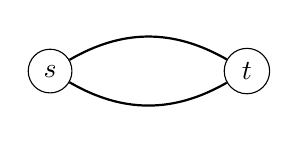
\begin{tikzpicture}[node distance = 2.5cm]
\node[white] (s) {$s$};
\node[white, right of=s] (t){$t$};

\draw[edge, bend right] (s) to (t);
\draw[edge, bend left] (s) to (t);
\end{tikzpicture} \end{center}

Jeder Serien-parallele Graph lässt sich durch Serien- und Parallelverbindungen konstruieren \cite{HasTam86}.
\end{definition}
\begin{definition}[Dekompostionsbaum eines Serien-parallelen Graphen]
Sei $G=(V,E)$ ein Serien-paralleler Graph. Der Dekompositionsbaum $T(G)$ von $G$ besteht aus Knoten, die alle Subbäume von $G$ repräsentieren.
Für jede Serien- oder Parallelverbindung durch die $G$ entstanden ist, entsteht eine Verzweigung in $T(G)$. Somit repräsentiert die Wurzel von $T(G)$ den gesamten Graphen $G$.
\end{definition}

In \cite{HasTam86} wurde mithilfe des Dekompositionsbaumes bewiesen, dass das \textit{UFLP} auf Serien-parallelen Graphen mit $n$ Knoten in $O(n^4)$ lösbar ist. Laut \cite{Gim17} wurde dies auch in \cite{Age90} bewiesen. Da diese Ausführung nur in russischer Sprache zugänglich war, konnte dies nicht überprüft werden. 

Der Algorithmus aus \cite{HasTam86} nutzt eine rekursive Funktion auf dem Dekompositionsbaum eines Serien-parallelen Graphen. So wird zunächst für die Blätter, die die einzelnen Komponenten des Graphen repräsentieren, die optimale Lösung berechnet und daraus dann die optimale Lösung für die Zusammengesetzten Komponenten. Dies wird fortgeführt, bis der gesamte Graph berücksichtigt wird. \\
Für die Rekursionsgleichung $h(q,j_s,j_t)$ auf dem Graphen $G=(V,E)$ ist $q$ ein Knoten aus~$T(G)$,~$G(q)$ der von $q$ repräsentierte Subgraph und $V_q$ die entsprechende Knotenmenge von $G(q)$. Außerdem sind $s(q)$ und $t(q)$ der Start- beziehungsweise Endknoten von $G(q)$. Als~$j_s$ und $j_t$ werden in der Gleichung die Facility Knoten, die $s(q)$ respektive $t(q)$ versorgen, bezeichnet.
Die Rekursionsgleichung für die Blätter lautet:
\[h(q,j_s,j_t) = \underset{S \subseteq V}{\min} \left\lbrace \sum_{w \in S} c_w + \sum_{w \in V(q)} \underset{u \in S}{\min} \{t_{wu}\} \right\rbrace\]

\noindent Für die inneren Knoten ist die Gleichung unterschiedlich für Serienverbindungen und Parallelverbindungen definiert. Die Hilfsfunktion $\delta(u,v,w)$ ist definiert als:
\[\delta(u,v,w) = \begin{cases} 1 & u=v=w \\ 0 & \text{sonst}
\end{cases}\]

\noindent Für Serienverbindungen $G(q) = S(G(q_1),G(q_2))$ von $G(q_1)$ und $G(q_2)$ mit~$s(q) = s(q_1)$, $t(q)~=~t(q_2)$ und $s(q_2) = t(q_1)$ gilt: 
\[h(q,j_s,j_t) = \underset{w \in V_q \cup \{j_s,j_t\}}{\min} \left\lbrace 
h(q_1,j_s,w) + h(q_2,w,j_t) - t_{t(q_1)w} - c_w - c_{j_s} \delta(j_s,j_t,w)
\right\rbrace\]

\noindent Für Parallelverbindungen $G(q) = P(G(q_1),G(q_2))$ mit $s(q) = s(q_1) = s(q_2)$,\\ $t(q) = t(q_1) = t(q_2)$ gibt es die Hilfsfunktion $\varepsilon$ mit $\varepsilon(u,v) = 1$, wenn $u \neq v$, ansonsten $\varepsilon(u,v) = 0$. Hier gilt:
\[h(q,j_s,j_t) = h(q_1,j_s,w) + h(q_2,w,j_t) - t_{s(q_1),j_s} - c_{j_s} - c_{j_t} \varepsilon(j_s,j_t) \]

\noindent So wird am Ende die optimale Lösung durch die Wurzel $r$ von $T(G)$ durch $\underset{j_s,j_t \in J}{\min} h(r,j_s,j_t)$ für den gesamten Graph berechnet. Die Berechnung aller Transportkosten benötigt $O(n^2)$ und die Berechnung der Rekursionsgleichung insgesamt $O(kn^3)$, wobei $k \in \N$ die Anzahl der Knoten in $T(G)$ ist \cite{HasTam86}. \\

\noindent Die Struktur der Serienparallelen Graphen findet sich vor allem bei elektrischen Schaltkreisen wieder \cite{RioSha42}.


\subsection{Das \textit{Capacitated Facility Location} Problem}
Im Unterschied zum \textit{UFLP} müssen beim \textit{CFLP} Kapazitäten für die Facilities eingehalten werden, die bestimmen, wie viele Klienten versorgt werden können. Dies macht das Problem schwerer zu lösen als das \textit{UFLP} \cite{Azi+20}.
In den Nebenbedingungen gibt es im Vergleich zum \textit{UFLP} folgende Veränderung: \\
Sei $d_i \in \N$ die Nachfrage des Klienten $i$ und $cap(j)$ die Kapazität der Facility $j$, dann muss für alle Facilities $j \in J$ gelten:
\[\sum_{i \in I} (d_i \cdot y_{ij}) \leq cap(j) \cdot x_j\]
Dies ersetzt die Nebenbedingung (3) aus \cref{def:uflp2} \cite{Hos21}. \\

Es konnte keine Literatur gefunden werden, die versucht einen der in dieser Arbeit untersuchten Algorithmen auf das \textit{CFLP} auf Bäumen anzuwenden. Der Algorighmus von Cornuejols et al. sollte hier allerdings daran scheitern, dass die Nebenbedingung, nach der für einen versorgten Klienten $i$ und die versorgende Facility $j$ alle Knoten $i' \in P(i,j)$ auch von $j$ versorgt werden müssen, nicht mehr gelten muss. Da die nächste Facility schon ihre Kapazität erreicht haben könnte, kann ein Klient auch von einer weiter entfernten Facility versorgt werden. Somit kann das Problem nicht mehr auf \textit{Tree Partition} reduziert werden. Es würden nicht-zusammenhängende Subbäume entstehen. \\
Für den Algorithmus von Kolen ist der Knackpunkt ein Ähnlicher. Im Algorithmus von Hoffman et al. würde eine Facility zu $S$ hinzugefügt werden, auch wenn sie nicht genügend Kapazität hätte. Es ist allerdings nicht ausgeschlossen, dass der Algorithmus entsprechend angepasst werden könnte.

\noindent Auch für das \textit{CFLP} gibt es polynomiell lösbare Fälle \cite{Azi+20}. Ein möglicher Fall, der nicht explizit auch für das \textit{UFLP} beschrieben wurde, ist das \textit{CFLP} auf Graphen mit beschränkter Baumweite.

\subsubsection{Graphen mit beschränkter Baumweite}\label{sec:treewidth}
Eine möglicherweise polynomiell lösbare Version des \textit{CFLP} ist die auf Graphen mit beschränkter Baumweite.
Die Baumweite eines Graphen bestimmt wie sehr dieser Graph einem Baum ähnlich ist \cite{FluGro06}. Ein Serien-paralleler Graph hat zum Beispiel Baumweite $2$ \cite{Kin11}. Ein Gittergraph mit $n$ Knoten hat eine Baumweite von $n$ \cite{Cyg+15}.

\begin{definition}[Baumweite \cite{FluGro06}]
Die \textit{Baumweite} eines Graphen $G$ ist das Minimum der Weiten der Baumzerlegungen von $G$. 
\end{definition}
 \pagebreak

\begin{definition}[Baumzerlegung \cite{FluGro06}]\label{def:treedecom}
Sei $G=(V,E)$ ein Graph. Eine Baumzerlegung von $G$ besteht aus einem Baum $T = (V_T,E_T)$ und den Mengen $(B_i)_{i \in V_T} \subseteq V$ für die gelten:
\begin{itemize}
\item Für jeden $v \in V$ gilt: $B^{-1}(v) = \{i \in V_T \mid v \in B_i\}$ ist nicht leer und mit $T$ verbunden.
\item Für jede Kante $\{v,u\} \in E$ existiert ein $i \in V_T$ mit $v,u \in B_i$.
\end{itemize}

\noindent Die Weite einer Zerlegung $(T,(B_i)_{i \in V_T})$ ist definiert als
\[\max\{|B_i|, i \in V_T\} - 1\]
Durch den Term $-1$ wird dafür gesorgt, dass die Weite der Baumzerlegung eines Baumes $1$ ist. 
\end{definition}

Das Ermittlen der Baumweite eines Graphen ist $\mathcal{NP}$-schwer \cite{Kin11}.
Für das kapazitierte \textit{FLP} wurde in \cite{Hos21} ein Algorithmus für Instanzen auf Graphen mit beschränkter Baumweite $k$ entwickelt. Dessen Worst-Case-Laufzeit liegt in
\[O\left(|V_T|^{O(1)} \cdot (B_{k+1} \cdot (2 \cdot \max\{cap(j) \mid j \in J\} + 1)^{k+1})^2 \cdot (k+1)^2 \right)\]
und ist somit von der Baumweite abhängig. Sobald die Baumweite also nicht konstant, sondern abhängig von der Eingabe ist, wäre dieser Algorithmus nicht mehr polynomiell.
Da die Arbeit noch nicht publiziert wurde, sollten dessen Ergebnisse allerdings mit Vorsicht gesehen werden. \\

Um das \textit{UFLP} in eine Instanz des \textit{CFLP} umzuwandeln, muss die Kapazität für jede Facility so gewählt werden, dass diese alle Klienten versorgen könnte. Da in der Definition des \textit{UFLP} für diese Arbeit keine Nachfrage benutzt wird, kann diese für jeden Klienten auf~$1$ gesetzt werden und die Kapazität der Facilities auf die Anzahl der Klienten. Somit ist der Algorithmus auch für das \textit{UFLP} anwendbar und damit könnte das \textit{UFLP} auf Graphen mit beschränkter Baumweite ebenfalls polynomiell lösbar sein.

\begin{example}{Baumzerlegung}{ex:treedecom}
Der folgende Graph ist eine Baumzerlegung des Graphen aus \Cref{ex:example}.
Da dieser bereits ein Baum war, ist die Baumweite der Zerlegung $2$. Das ist erkenntlich daran, dass für jeden Knoten der Zerlegung höchstens zwei Knoten aus dem ursprünglichen Graph verwendet wurden. \\

\centering
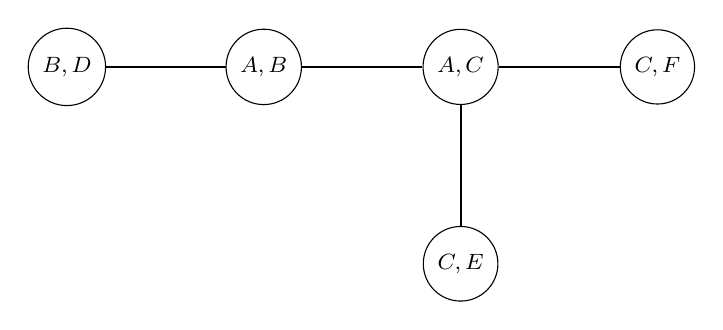
\begin{tikzpicture}[node distance=2.5cm]
\node[white] (AB) {\footnotesize $A,B$};
\node[white, left of=AB] (BD) {\footnotesize $B,D$};
\node[white, right of=AB] (AC) {\footnotesize $A,C$};
\node[white, below of=AC] (CE) {\footnotesize $C,E$};
\node[white, right of=AC] (CF) {\footnotesize $C,F$};

\draw[edge] (AB) -- (BD);
\draw[edge] (AB) -- (AC);
\draw[edge] (AC) -- (CE);
\draw[edge] (AC) -- (CF);
\end{tikzpicture}
\end{example} 


\section{Charakteristika der Algorithmen}\label{sec:characteristics}
Nachdem nun zwei Algorithmen und ihre Optimalität ausführlich ergründet wurden, stellt sich die Frage, warum das \textit{UFLP} auf Bäumen und auch auf anderen Strukturen einfacher zu lösen ist als auf generellen Graphen. \\
Die naheliegenden Eigenschaften eines Baumes sind seine azyklische Struktur und die daraus hervorgehenden eindeutigen Pfade zwischen zwei Knoten. Da allerdings auch das \textit{UFLP} auf Serien-parallelen Graphen, die diese beiden Eigenschaften nicht erfüllen, in polynomieller Zeit lösbar ist, können Diese nicht ausschlaggebend dafür sein, dass diese Probleme in $\mathcal{P}$ liegen. \\ 
 
Eine Eigenschaft, die die beiden Algorithmen gleich haben und auch \cref{sec:els,sec:jones,sec:spgraph,sec:treewidth} beinhalten, ist eine feste, von der Topologie des Graphen abhängigen Ordnung, die in ihrer Länge höchstens polynomiell von der Eingabe abhängig ist.
Nach dieser Reihenfolge, ob iterativ oder rekursiv, werden Teillösungen gesucht und im Anschluss zusammengefügt. 

Ein weiterer Ansatz ist, sich anzuschauen wie die Baumweite eines Graphen bestimmt wird.
Die Klasse der Graphen mit beschränkter Baumweite beinhaltet alle Bäume und Serien-parallelen Graphen \cite{Cyg+15}, somit ist hier am ehesten eine Abgrenzung zu den generellen Graphen zu finden.
Nach \cref{def:treedecom} ist die Baumweite abhängig davon, wie viele Knoten bei der Dekomposition zu Einem vereinigt wurden. Ist die Baumweite beschränkt, ist nach \cite{Hos21} auch die Laufzeitkomplexität des Algorithmus polynomiell. Dies ist bei einer unbeschränkten Baumweite nicht mehr der Fall. 
Wovon genau die Baumweite abhängig ist, bleibt allerdings Gegenstand der zukünftigen Forschung.

\pagebreak

\section{Fazit}\label{sec:fazit}
%Hier ist die Arbeit zu Ende. Ich finde, dass die Arbeit vorzüglich gelungen ist und ich eine 1.0 verdient habe. Danke! 
%Ich möchte an dieser Stelle noch meiner Freundin Melinda Heinkes danken, die große Teile meiner Bachelorarbeit geistig bereichert hat und ohne die ich nicht der Mann wäre, der ich heute bin. Amen!
In dieser Arbeit wurden die Algorithmen von Kolen und Cornuejols et al. für das \textit{Uncapacitated Facility Location} Problem umfassend erklärt und analysiert. Der Algorithmus von Kolen nutzt eine Umformulierung in ein \textit{Covering} Problem, die Eigenschaften der damit verbundenen Nebenbedingungsmatrix und die duale Lösung um einen polynomiellen Algorithmus zu erstellen, der das Problem in $O(n^3)$ Schritten für einen Baum mit $n$ Knoten löst. \\
Cornuejols et al. nutzen eine Rekursionsgleichung, die für jede Kombination aus versorgtem Klienten und versorgender Facility die Kosten errechnet und von den Blättern zur Wurzel hin die optimalen Lösungen kombiniert. Dies ermöglicht die Berechnung in $O(n^2)$ Schritten.
Die Argumentation für die Optimalität der Lösung erfolgt auch hier über das duale Problem.\\

Aus den Recherchen zu diesen Algorithmen und einigen anderen polynomiell lösbaren Fällen ließen sich mehrere Gründe ableiten, die dafür sorgen könnten, dass die Baumstruktur das \textit{UFLP} einfacher macht.
Ein Grund ist die Verwendung einer festen, von der Topologie abhängigen Ordnung, die in ihrer Länge höchstens polynomiell von der Größe des Graphen abhängig ist. Der Andere liegt in der Definition der Baumweite. Auf Graphen mit beschränkter Baumweite kann das \textit{Capacitated Facility Location} Problem mit dem Algorithmus von \cite{Hos21} womöglich polynomiell gelöst werden. Da das \textit{UFLP} als Spezialfall des \textit{CFLP} formuliert werden kann, funktioniert dieser Algorithmus auch hierfür, ist aber in seiner Komplexität von der Baumweite abhängig. \\
Insgesamt ist dieses Thema eines, das Anlass zu reger Forschung bietet, da die Anwendungen für das \textit{UFLP} vielseitig sind. Eine möglichst breite Klasse von Graphen, auf denen dieses Problem polynomiell lösbar ist, oder eine Verbesserung der bisherigen Algorithmen  kann den Aufwand für das Lösen komplexer Instanzen deutlich verringern.
Auch wenn die hier untersuchten Algorithmen schon mehrere Dekaden alt sind, sieht man durch \cite{Hos21}, dass die Forschung auf diesem Gebiet nicht abgeschlossen ist und neue Erkenntnisse hervorbringt. 


\pagebreak
\pagenumbering{Roman}
\addcontentsline{toc}{section}{Literatur}
\printbibliography
\pagebreak

\begin{appendix}
\addcontentsline{toc}{part}{Anhang}
\section{Theoretische Grundlagen}\label{sec:theorie}
In diesem Abschnitt werden die Konzepte erklärt, die benötigt werden um die Arbeit voll umfänglich zu verstehen.

\subsection{Graphen} \label{sec:graphen}

\begin{wrapfigure}{r}{0.5\textwidth}
\vspace*{-0.5cm}
\centering
\begin{example}{Graph}{ex:graph}
\centering
\caption{Beispiel eines azyklischen, ungerichteten Graphen mit $V=\{v_A,v_B,v_C\}$ und $E=\{\{v_A,v_B\},\{v_A,v_C\}\}$\\}
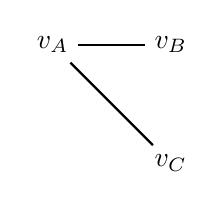
\begin{tikzpicture}[node distance=1.5cm]
	\node[blank] (A) {$v_A$};
	\node[blank, right of=A] (B) {$v_B$};
	\node[blank, below of=B] (C) {$v_C$};
		
	
	\draw[edge] (A) -- (B);
	\draw[edge] (A) -- (C);
\end{tikzpicture}
\end{example}
\end{wrapfigure}
Ein Graph besteht aus Knoten und Kanten. Die Knotenmenge wird beschrieben durch $V$ und die Kanten als~$E$. Eine Kante verbindet zwei Knoten, weshalb sie als $\{v_1,v_2\} \in E$ mit $v_1,v_2 \in~V$ geschrieben wird bei ungerichteten Graphen und als $(v_1,v_2) \in E$ bei gerichteten Graphen. \\
Ein gerichteter Graph hat Kanten, die nur in eine Richtung verwendet werden können, also $(v_1,v_2)$ nur von $v_1$ zu $v_2$. Intuitiv könnte man sich Kanten als Straßen vorstellen und eine gerichtete Kante als Einbahnstraße.\\

\begin{definition}[Pfad]
Sei $G=(V,E)$ ein Graph und $v_1,v_2 \in V$ zwei Knoten darin. \\
$P(v_1,v_2) = v_1,...,v_2$ ist ein Pfad in $G$, wenn für aufeinanderfolgende $v_i,v_j$ in $P(v_1,v_2)$ gilt: $\{v_i,v_j\} \in E$ bzw. $(v_i,v_j) \in E$
\end{definition}

\subsubsection{Bäume} \label{sec:bäume}
Ein Baum ist ein Graph $G = (V,E)$ mit den Eigenschaften, dass dieser ungerichtet und azyklisch ist. 
Aus diesen beiden Eigenschaften folgt, dass für jedes beliebige Knoten-\\paar~$v_1,v_2 \in~V$ nur ein Pfad existiert, der die Beiden verbindet, also 
$\forall v_1,v_2 \in V$  mit~$P(v_1,v_2)$ ist gültiger Pfad in $G$: \[\nexists P'(v_1,v_2) \neq P(v_1,v_2) \text{ mit }P'(v_1,v_2) \text{gültiger Pfad in }G. \] 
Der Graph in \Cref{ex:graph} ist ein Baum. 

\subsection{P und NP}
Die Komplexität von lösbaren Problemen wird in der Informatik grob in zwei Klassen eingeteilt. Die Probleme, die \glqq einfach\grqq{} zu lösen sind, und die, die man (noch) nicht \glqq einfach\grqq{} lösen kann. Einfach bedeutet hier, dass es eine Methode gibt, die das Problem in polynomieller Zeit zur Eingabelänge löst. Diese Klasse an Problemen nennt sich $\mathcal{P}$.
Probleme, dessen Lösungen sich in polynomieller Zeit überprüfen lassen, gehören zur Klasse $\mathcal{NP}$. Diese Klasse ist formell so definiert, dass die Probleme in ihr auf einer nicht-deterministischen Turingmaschine in polynomieller Zeit gelöst werden können \cite[S. 46]{Pap94}. Somit gilt auch: $\mathcal{P} \subseteq \mathcal{NP}$. Es wird allgemein angenommen, dass $\mathcal{P} \neq \mathcal{NP}$ gilt \cite{Cor+90}.

\subsection{Lineare Programme} \label{sec:lps}
Ein Lineares Programm besteht aus einer Zielfunktion und Nebenbedingungen.
Allgemein hat eine Zielfunktion die Form
\[\min/\max c^Tx\]
wobei $x$ sogenannte Entscheidungsvariablen sind und $c$ gegebene Werte.
Die Nebenbedingungen haben die Form
\[a_i^Tx \circ b_i\]
wobei $\circ \in \{=,\leq,\geq\}$ ist und $a_i$ und $b_i$ gegebene Werte sind.
Den Vektor $b$ nennt man dabei Beschränkungen und die Matrix $A= (a_{ij})$ Nebenbedingungsmatrix. \\
Dazu gehören im Allgemeinen Nebenbedingungen, die festlegen welche Werte die Entscheidungsvariablen annehmen können (z.B. $x \in \{0,1\}$ oder $x \geq 0$). \\
Ziel ist es, die Zielfunktion zu optimieren, wobei alle Nebenbedingungen eingehalten werden.


\subsubsection{Dualität} \label{sec:dual}
Für ein Lineares Programm $\min c^Tx$ unter $Ax \geq b, x \geq 0$ wird das \textit{Duale LP} definiert als:
\[\max b^Ty \text{ unter } A^Ty \leq c, y \geq 0 \quad \text{ \cite{Gal89}}\] 


\begin{theorem}[Schwacher Dualitätssatz]\label{thm:schwachedualitaet}
Sei $x$ eine gültige Lösung für ein primales Problem und $y$ eine gültige Lösung für das zugehörige duale Problem. Wenn das primale LP ein Maximierungsproblem ist, gilt: 
\[c^Tx \leq y^Tb.\]
Ist das primale ein Minimierungsproblem gilt analog: $y^Tb \leq c^Tx$.
\end{theorem}
\begin{proof}
Es gelten: $y^TA \geq c^T \text{ und } x\geq 0$, sowie $Ax\leq b \text{ und } y \geq 0$.\\
Daraus folgt: $c^Tx \leq y^TAx \leq y^Tb$ und somit $c^Tx \leq y^Tb$.
\end{proof}



\begin{theorem}[Starke Dualität]\label{thm:strongduality}
Sei $x$ eine Lösung für ein LP und $y$ eine Lösung für das dazugehörige duale LP. Wenn $c^Tx = y^Tb$, dann sind $x$ und $y$ die optimalen Lösungen für ihr jeweiliges LP.
\end{theorem}
\begin{proof}
Es wird angenommen, dass das primale LP ein Maximierungsproblem und das duale LP ein Minimierungsproblem ist. Die Argumentation erfolgt analog im umgekehrten Fall.\\
Durch den \textit{schwachen Dualitätssatz} (\cref{thm:schwachedualitaet}) gilt: Für alle Lösungen~$x$ für ein LP und~$y$ für das dazugehörige duale LP: $y^Tb \geq c^Tx$.\\
Sollte $x$ keine optimale Lösung für das primale Problem sein, müsste ein $x'$ existieren mit~$c^Tx'~>~c^Tx$. Da allerdings $y^Tb = c^Tx$ widerspräche dies dem schwachen Dualitätssatz.\\
Sollte $y$ keine optimale Lösung für das duale Problem sein, müsste ein $y'$ existieren\\ mit $y'^Tb <~y^Tb$. Da allerdings $y^Tb = c^Tx$, widerspräche dies dem schwachen Dualitätssatz.
\end{proof}


\subsubsection{Komplentaritätsbedingung}\label{sec:compslack}

Die Komplementaritätsbedingung wird auch komplementärer Schlupf beziehungsweise complementary slackness genannt und ist eine Optimalitätsvoraussetzung für Lineare Programme. \\

Seien ein primales Problem $\min c^Tx$ unter $Ax = b, x \geq 0$ und das dazugehörige duale Problem $\max b^T\lambda$ unter $A^T\lambda + s = c, s \geq 0$ gegeben, wobei mit $s$ eine Schlupfvariable genutzt wird. \\
Nach \cite[86]{GeiKan02} sind folgende Aussagen äquivalent:
\begin{itemize}
\item[(a)] Das primale Problem hat eine Lösung $x^*$
\item[(b)] Das duale Problem hat eine Lösung $(\lambda^*, s^*)$
\item[(c)] Es gibt eine Lösung $(x^*,\lambda^*,s^*)$ für:
\begin{align*}
A^T\lambda + s &= c&& \\
Ax &= b&& \\
x_is_i &= 0 \quad i = 1,...,n &&\\
x,s &\geq  0&&
\end{align*}
\end{itemize}
Die Gleichungen aus (c) lassen sich umformen zu:
\begin{align*}
A^T\lambda + s - c &= 0&& \\
Ax -b &= 0&& \\
x_is_i &= 0 \quad i = 1,...,n &&\\
x,s &\geq  0&&
\end{align*}


\end{appendix}
%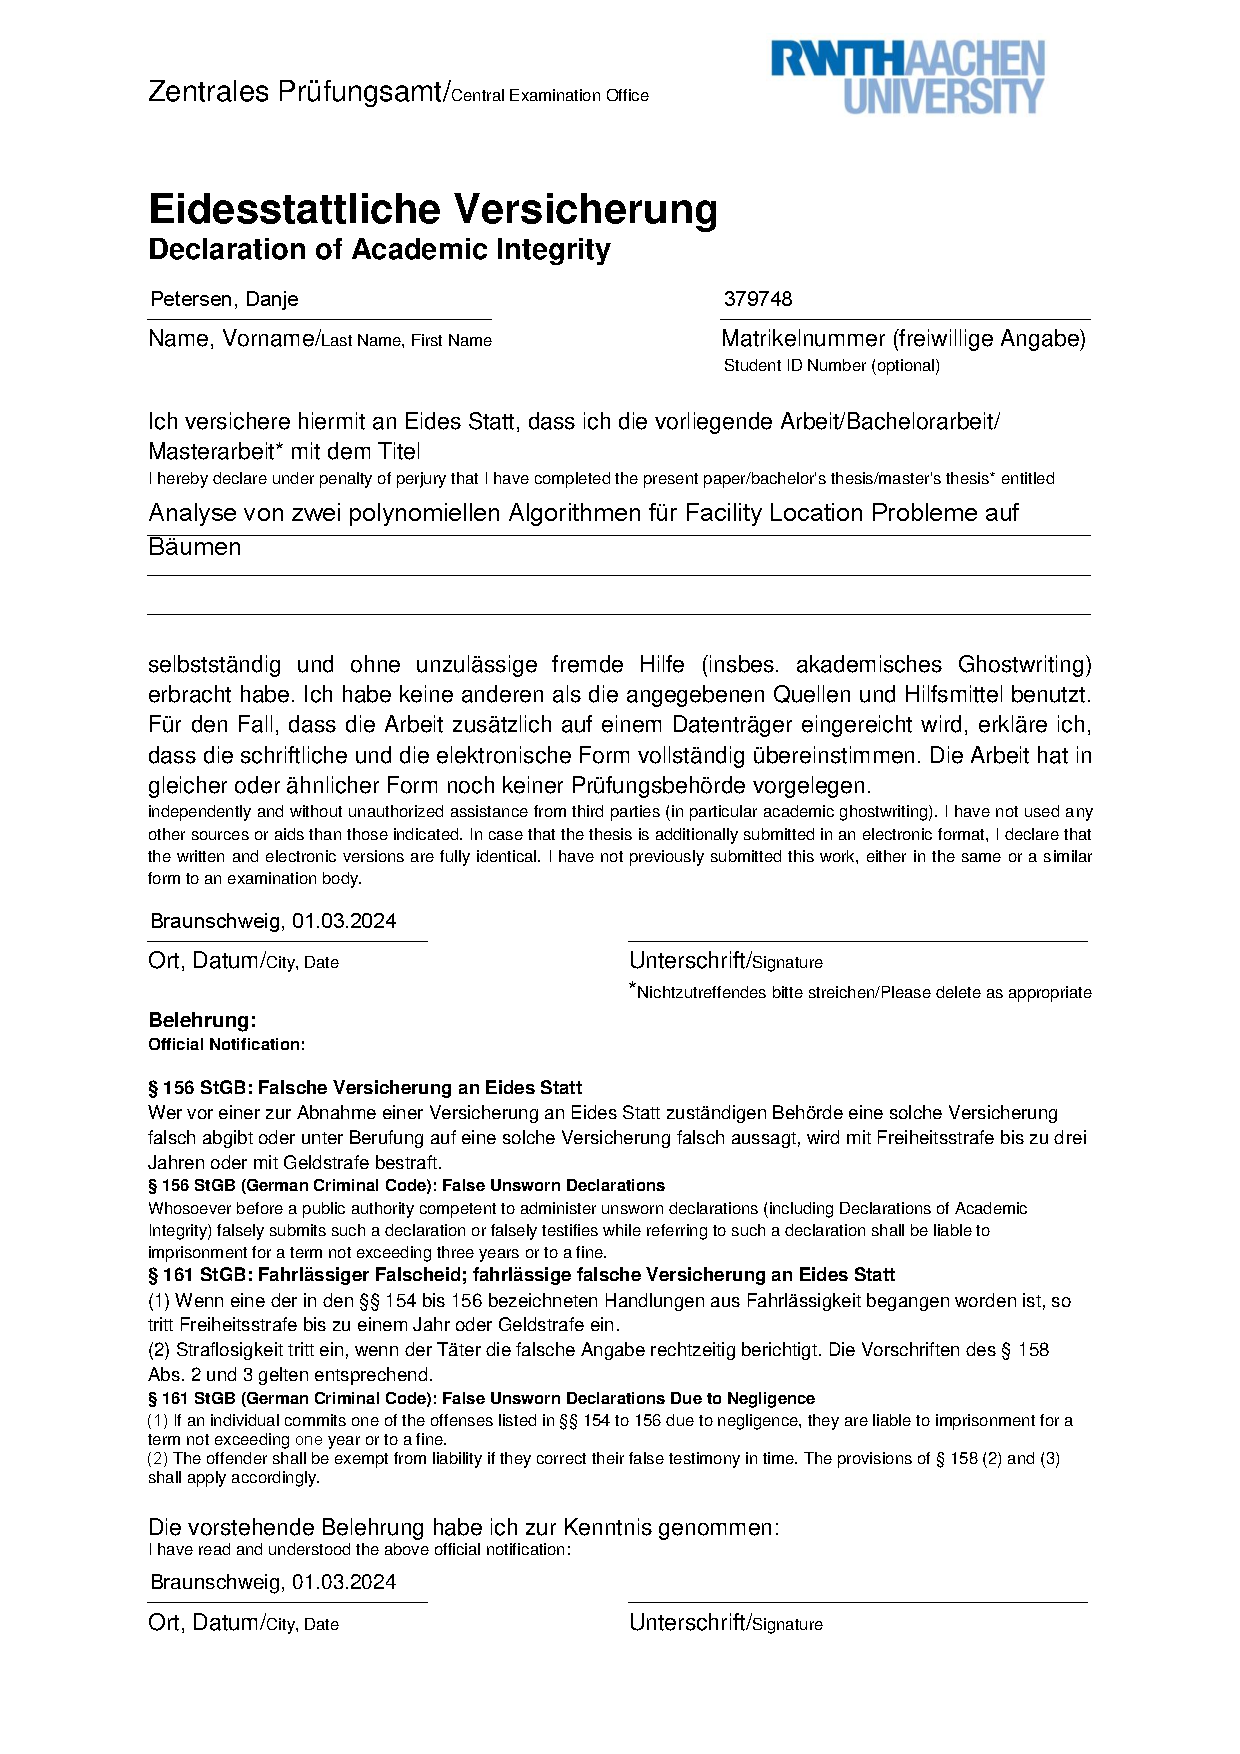
\includepdf{includes/eidesstattlichevers.pdf}

\end{document}

